% =========================================================
%  Chapter 6 — Homojunctions, Heterojunctions, and Optical Gain
%  Source: Dr. George's Lectures (Lecture 2)
%  Style: student-voice notes matching the personal style guide
% =========================================================

% ------------------------------------------------------------------
\section{Picking Up Where We Left Off}
% ------------------------------------------------------------------

The previous chapter established the fundamental physics needed to achieve optical gain in a semiconductor: we need two separate quasi-Fermi levels $E_{fn}$ and $E_{fp}$, separated by enough energy to satisfy the Bernard-Duraffourg condition $E_{fn} - E_{fp} > h\nu > E_g$. We also established that a homojunction — a simple PN junction made of a single semiconductor material — can in principle achieve this, but at the cost of an impractically high threshold current density. Before we can understand why the modern laser diode solved this problem so elegantly, we need to go deeper into the homojunction: to quantify exactly how the depletion region forms, what determines its width, and how optical gain connects to the carrier statistics on a state-by-state basis. Only then can we properly appreciate what the double heterostructure achieves.

% ------------------------------------------------------------------
\section{The Homojunction at Equilibrium}
% ------------------------------------------------------------------

\subsection{Fermi Level Alignment and the Built-In Potential}

Before two differently-doped regions of the same semiconductor material are brought into contact, each has its own Fermi level: the n-side has $E_f$ lying close to the conduction band (reflecting its excess electrons), and the p-side has $E_f$ lying close to the valence band (reflecting its excess holes).

The moment contact is made, a fundamental rule of thermodynamics takes over: at thermal equilibrium, the Fermi level must be flat and continuous throughout the entire structure. Electrons diffuse from the n-side (where they are abundant) into the p-side, and holes diffuse in the opposite direction. This carrier diffusion leaves behind fixed, ionised donor and acceptor atoms in what becomes the \textbf{depletion region} — a layer stripped of free carriers. This fixed charge creates a built-in electric field pointing from n to p, which opposes further diffusion and ultimately halts the net flow.

The resulting electrostatic potential difference across the junction is the \textbf{built-in (contact) potential} $V_0$. By definition, the energy difference between the conduction bands on either side is $E_c^p - E_c^n = qV_0$.

To find its value, we apply the equilibrium condition that the electron concentration on the n-side ($n_{n0}$) and the p-side ($n_{p0}$) must be governed by the exact same flat Fermi level $E_f$:
\begin{align*}
    n_{n0} &= N_c \exp\!\left(-\frac{E_c^n - E_f}{k_B T}\right) \approx N_d \\
    n_{p0} &= N_c \exp\!\left(-\frac{E_c^p - E_f}{k_B T}\right) \approx \frac{n_i^2}{N_a}
\end{align*}

Taking the ratio of these two concentrations isolates the energy difference:
\begin{align*}
    \frac{N_d}{n_i^2 / N_a} &= \frac{\exp\!\left(-(E_c^n - E_f)/k_B T\right)}{\exp\!\left(-(E_c^p - E_f)/k_B T\right)} \\
    \frac{N_d N_a}{n_i^2} &= \exp\!\left(\frac{E_c^p - E_c^n}{k_B T}\right) = \exp\!\left(\frac{qV_0}{k_B T}\right)
\end{align*}

Taking the natural logarithm of both sides yields the final expression:
\begin{keyresult}
    \begin{equation}
        V_0 = \frac{k_B T}{q}\,\ln\!\left(\frac{N_d\,N_a}{n_i^2}\right)
    \end{equation}
\end{keyresult}
where:
\begin{itemize}
    \item $V_0$: the built-in potential (Volts) — the height of the electrostatic barrier that forms spontaneously at the junction.
    \item $N_d$, $N_a$: the donor and acceptor doping concentrations (m$^{-3}$) on the n and p sides respectively.
    \item $n_i$: the intrinsic carrier concentration (m$^{-3}$), which was derived in the previous chapter as $n_i^2 = N_c N_v \exp(-E_g/k_B T)$.
    \item $k_B T/q$: the thermal voltage, approximately $26\,\text{mV}$ at room temperature.
\end{itemize}

\begin{figure}[H]
    \centering
    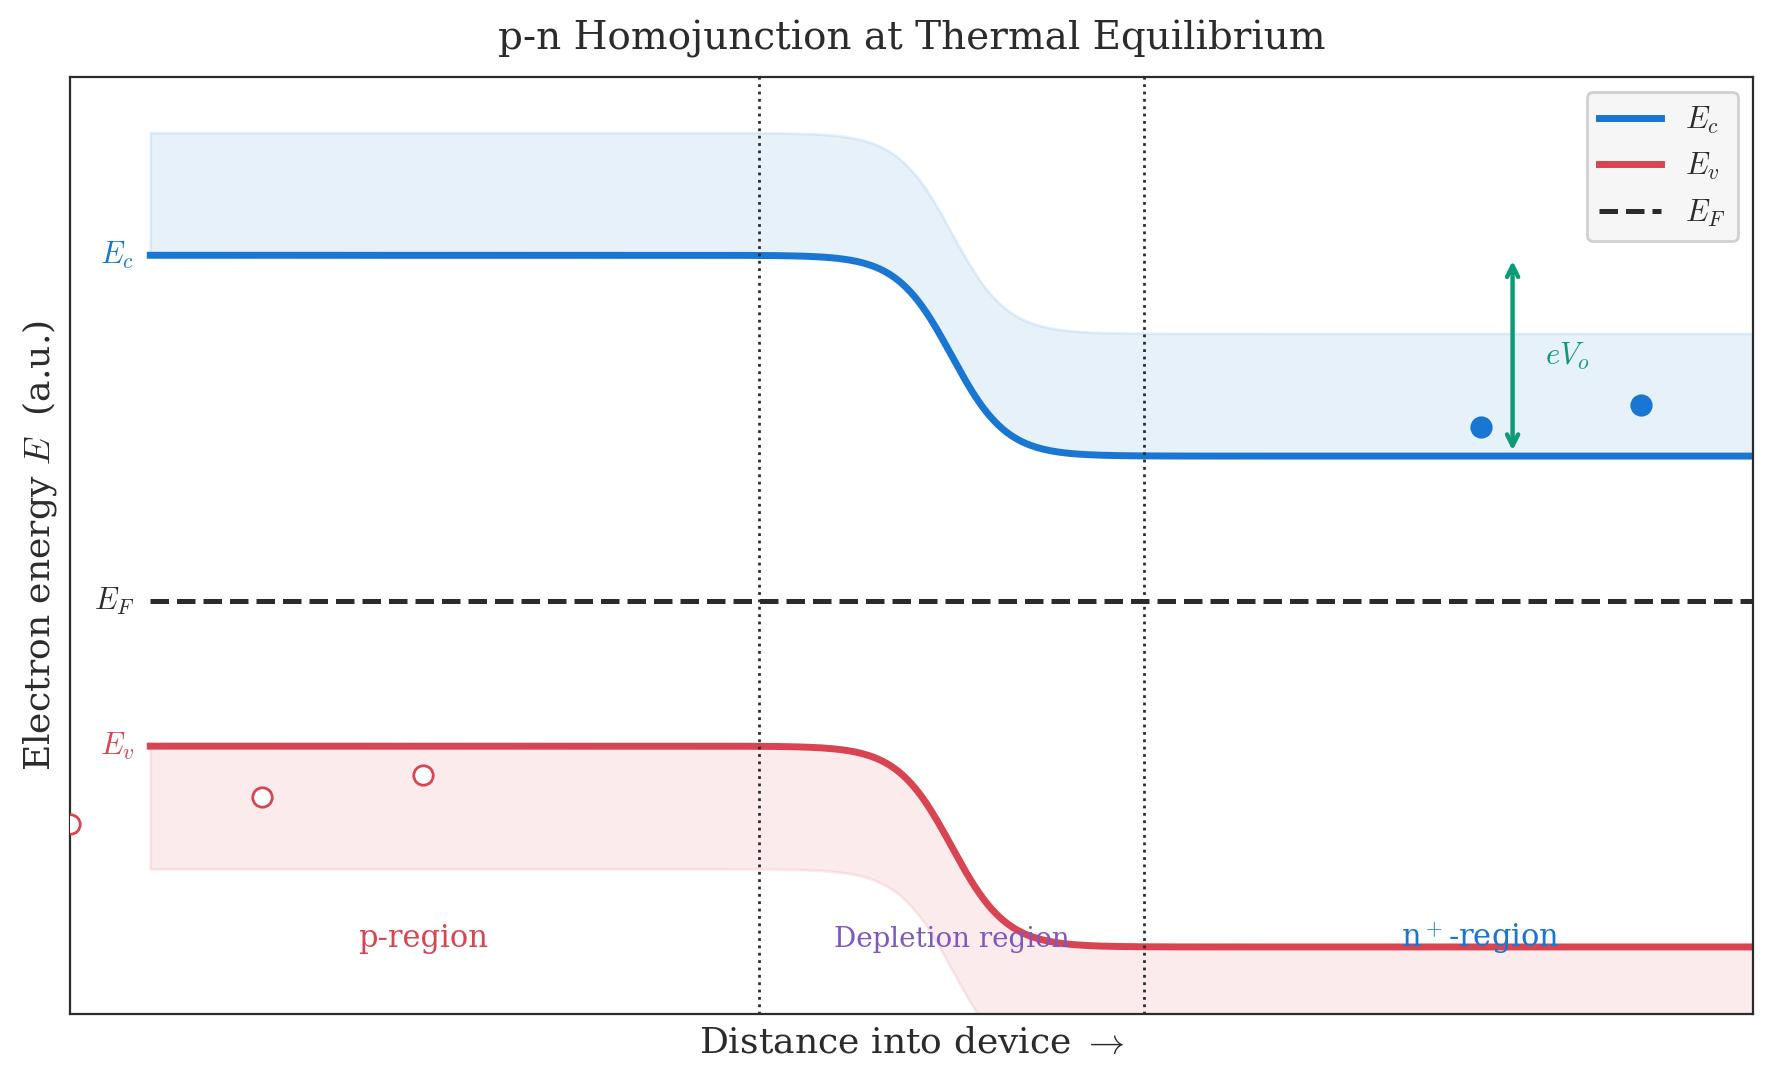
\includegraphics[width=0.65\textwidth]{Figures/Chapter 6/homojunction_equilibrium.jpg}
    \caption{p-n Homojunction Band Diagram at Thermal Equilibrium}
\end{figure}

Notice the logarithmic dependence: heavier doping on either side pushes the Fermi levels further toward the band edges, increasing the potential difference. At room temperature with typical doping densities of $10^{17}$--$10^{18}\,\text{cm}^{-3}$, $V_0$ is typically in the range of $0.5$--$1.5\,\text{V}$ for GaAs.

\subsection{Majority and Minority Carrier Concentrations}

With the equilibrium Fermi level known, we can write down the carrier populations on each side using the results from the previous chapter.

In the \textbf{n-doped region}, donors are essentially fully ionised, so the majority electron concentration is simply set by the doping:
\begin{equation*}
    n_{n0} = N_d, \qquad p_{n0} = \frac{n_i^2}{N_d}
\end{equation*}
The minority hole density $p_{n0}$ is suppressed far below $n_i$ because the mass-action law $np = n_i^2$ must be conserved — pushing $n$ up forces $p$ down proportionally.

In the \textbf{p-doped region}, acceptors are fully ionised, so holes are the majority carrier:
\begin{equation*}
    p_{p0} = N_a, \qquad n_{p0} = \frac{n_i^2}{N_a}
\end{equation*}

These minority carrier densities are not just theoretical curiosities. In fact, understanding their extreme scarcity at equilibrium is central to understanding how optoelectronic devices like LEDs and laser diodes function.

To produce meaningful optical emission, an electron must recombine with a hole, releasing its energy as a photon. This requires a high concentration of \emph{both} electrons and holes existing in the exact same physical space simultaneously.

Under thermal equilibrium (no applied voltage), the mass-action law guarantees this condition is never met:
\begin{itemize}
    \item \textbf{On the p-side:} There is an ocean of majority holes, but practically zero minority electrons.
    \item \textbf{On the n-side:} There is an ocean of majority electrons, but practically zero minority holes.
\end{itemize}

If we consider an electron sitting on the p-side, it has plenty of holes to recombine with. However, because electrons are minority carriers here, their equilibrium concentration is so low that almost no light is produced.

This low equilibrium concentration is precisely why we must actively inject carriers with current. When a forward bias is applied, we physically push electrons from the n-side over the junction into the p-side, where they instantly become minority carriers. Simultaneously, holes are injected into the n-side.

This injection floods the regions with minority carriers, creating a massive, non-equilibrium population of both electrons and holes in the same place. Because they are no longer constrained by the equilibrium mass-action law, they rapidly recombine in massive numbers, yielding the bright optical emission that powers modern LEDs.

% ------------------------------------------------------------------
\section{Depletion Region Analysis}
% ------------------------------------------------------------------

\subsection{Charge Neutrality and Individual Widths}

The depletion region extends a distance $W_{p0}$ into the p-side and $W_{n0}$ into the n-side. Because the entire structure must remain electrically neutral, the total fixed positive charge on the n-side must exactly equal the total fixed negative charge on the p-side. Since the charge density on each side is simply $qN_d$ and $qN_a$ respectively:
\begin{keyresult}
    \begin{equation}
        W_{p0}\,N_a = W_{n0}\,N_d
    \end{equation}
\end{keyresult}

This single equation contains important physics: the depletion region extends further into the \emph{lightly doped} side. If $N_a \gg N_d$, then $W_{p0} \ll W_{n0}$ — the depletion region is almost entirely on the n-side, because the lightly doped n-side needs a large volume of charge to balance the dense acceptor charge on the p-side. This asymmetry is exploited in practice to concentrate the depletion region (and hence the gain region) on one side of the junction.

\subsection{Building Up to the Total Depletion Width}

We start from Poisson's equation in 1D, which relates the electrostatic potential $V(x)$ and the electric field $\mathcal{E}(x) = -\frac{dV}{dx}$ to the charge density $\rho(x)$:
\begin{equation*}
    \frac{d\mathcal{E}}{dx} = \frac{\rho(x)}{\epsilon}
\end{equation*}
In the depletion approximation, we assume the free carriers are completely swept out, leaving only the fixed ionized dopants. The charge density profile is:
\begin{equation*}
    \rho(x) = 
    \begin{cases}
        -q N_a & \text{for } -W_{p0} \le x < 0 \quad (\text{p-side}) \\
        q N_d & \text{for } 0 < x \le W_{n0} \quad (\text{n-side})
    \end{cases}
\end{equation*}
Integrating Poisson's equation on the n-side ($0 \leq x \leq W_{n0}$) with the boundary condition that the electric field must vanish at the depletion boundary ($\mathcal{E}(W_{n0}) = 0$):
\begin{equation*}
    \int_{\mathcal{E}(x)}^{0} d\mathcal{E}' = \int_x^{W_{n0}} \frac{qN_d}{\epsilon}\,dx' \implies -\mathcal{E}(x) = \frac{qN_d}{\epsilon}(W_{n0} - x) \implies \mathcal{E}(x) = \frac{qN_d}{\epsilon}(x - W_{n0})
\end{equation*}
Symmetrically, integrating on the p-side ($-W_{p0} \leq x < 0$) with the boundary condition $\mathcal{E}(-W_{p0}) = 0$:
\begin{equation*}
    \int_0^{\mathcal{E}(x)} d\mathcal{E}' = \int_{-W_{p0}}^x -\frac{qN_a}{\epsilon}\,dx' \implies \mathcal{E}(x) = -\frac{qN_a}{\epsilon}(x + W_{p0})
\end{equation*}
Since the electric field must be continuous at the metallurgical junction ($x=0$), equating the two expressions yields the peak field magnitude at $x=0$:
\begin{equation*}
    \mathcal{E}_0 = -\frac{qN_d\,W_{n0}}{\epsilon} = -\frac{qN_a\,W_{p0}}{\epsilon}
\end{equation*}
which directly recovers the charge neutrality condition $N_d W_{n0} = N_a W_{p0}$.

To find the electrostatic potential profile $V(x)$, we integrate the electric field $\frac{dV}{dx} = -\mathcal{E}(x)$. We set the potential on the p-side boundary as our reference, $V(-W_{p0}) = 0$.
Integrating across the p-side ($-W_{p0} \leq x < 0$):
\begin{equation*}
    V(x) = \int_{-W_{p0}}^x -\mathcal{E}(x')\,dx' = \int_{-W_{p0}}^x \frac{qN_a}{\epsilon}(x' + W_{p0})\,dx' = \frac{qN_a}{2\epsilon}(x + W_{p0})^2
\end{equation*}
Thus, the potential drop across the p-side depletion region is:
\begin{equation*}
    V_p \equiv V(0) = \frac{qN_a W_{p0}^2}{2\epsilon}
\end{equation*}
Next, integrating across the n-side ($0 < x \le W_{n0}$):
\begin{equation*}
    V(x) - V(0) = \int_0^x -\mathcal{E}(x')\,dx' = \int_0^x -\frac{qN_d}{\epsilon}(x' - W_{n0})\,dx' = -\frac{qN_d}{\epsilon}\left(\frac{x^2}{2} - W_{n0} x\right)
\end{equation*}
The potential drop across the n-side depletion region is $V_n \equiv V(W_{n0}) - V(0)$:
\begin{equation*}
    V_n = \frac{qN_d W_{n0}^2}{2\epsilon}
\end{equation*}
The total built-in potential $V_0$ is the sum of these potential drops:
\begin{equation*}
    V_0 = V_p + V_n = \frac{q}{2\epsilon}\left(N_a W_{p0}^2 + N_d W_{n0}^2\right)
\end{equation*}
Alternatively, because the electric field profile is perfectly triangular, the total potential $V_0 = \int_{-W_{p0}}^{W_{n0}} |\mathcal{E}(x)|\,dx$ is simply the area of the field triangle ($\frac{1}{2} \times \text{base} \times \text{height}$):
\begin{equation*}
    V_0 = \frac{1}{2} W_0 |\mathcal{E}_0|
\end{equation*}
where $W_0 = W_{n0} + W_{p0}$ is the total depletion width. Substituting the peak field magnitude $|\mathcal{E}_0| = \frac{q N_d W_{n0}}{\epsilon}$:
\begin{equation*}
    V_0 = \frac{1}{2} W_0 \left( \frac{qN_d W_{n0}}{\epsilon} \right)
\end{equation*}

However, from the charge neutrality condition ($W_{p0}N_a = W_{n0}N_d$) and the fact that $W_0 = W_{n0} + W_{p0}$, we can express the n-side width purely as a fraction of the total width:
\begin{align*}
    W_{n0} &= W_0 - W_{p0} \\
    W_{n0} &= W_0 - W_{n0}\frac{N_d}{N_a} \\
    W_{n0} &= \frac{N_a}{N_a + N_d} W_0
\end{align*}

Substituting this expression for $W_{n0}$ back into the potential equation:
\begin{align*}
    V_0 &= \frac{1}{2} W_0 \frac{qN_d}{\epsilon} \left( \frac{N_a}{N_a + N_d} W_0 \right) \\
    V_0 &= \frac{1}{2}\frac{q}{\epsilon}\frac{N_a N_d}{N_a + N_d} W_0^2
\end{align*}

Finally, rearranging this to solve for the total depletion width $W_0$:
\begin{keyresult}
    \begin{equation}
        W_0 = \sqrt{\frac{2\epsilon}{q}\cdot\frac{N_a + N_d}{N_a N_d}\cdot V_0}
    \end{equation}
\end{keyresult}

Substituting the full expression for $V_0$ from above:
\begin{equation*}
    W_0 = \sqrt{\frac{2\epsilon}{q}\cdot\frac{k_B T}{q}\left(\frac{1}{N_a}+\frac{1}{N_d}\right)\ln\!\frac{N_d N_a}{n_i^2}}
\end{equation*}

The individual widths then follow directly from charge neutrality:
\begin{equation*}
    W_{p0} = \frac{W_0\,N_d}{N_a + N_d}, \qquad W_{n0} = \frac{W_0\,N_a}{N_a + N_d}
\end{equation*}

\begin{figure}[H]
    \centering
    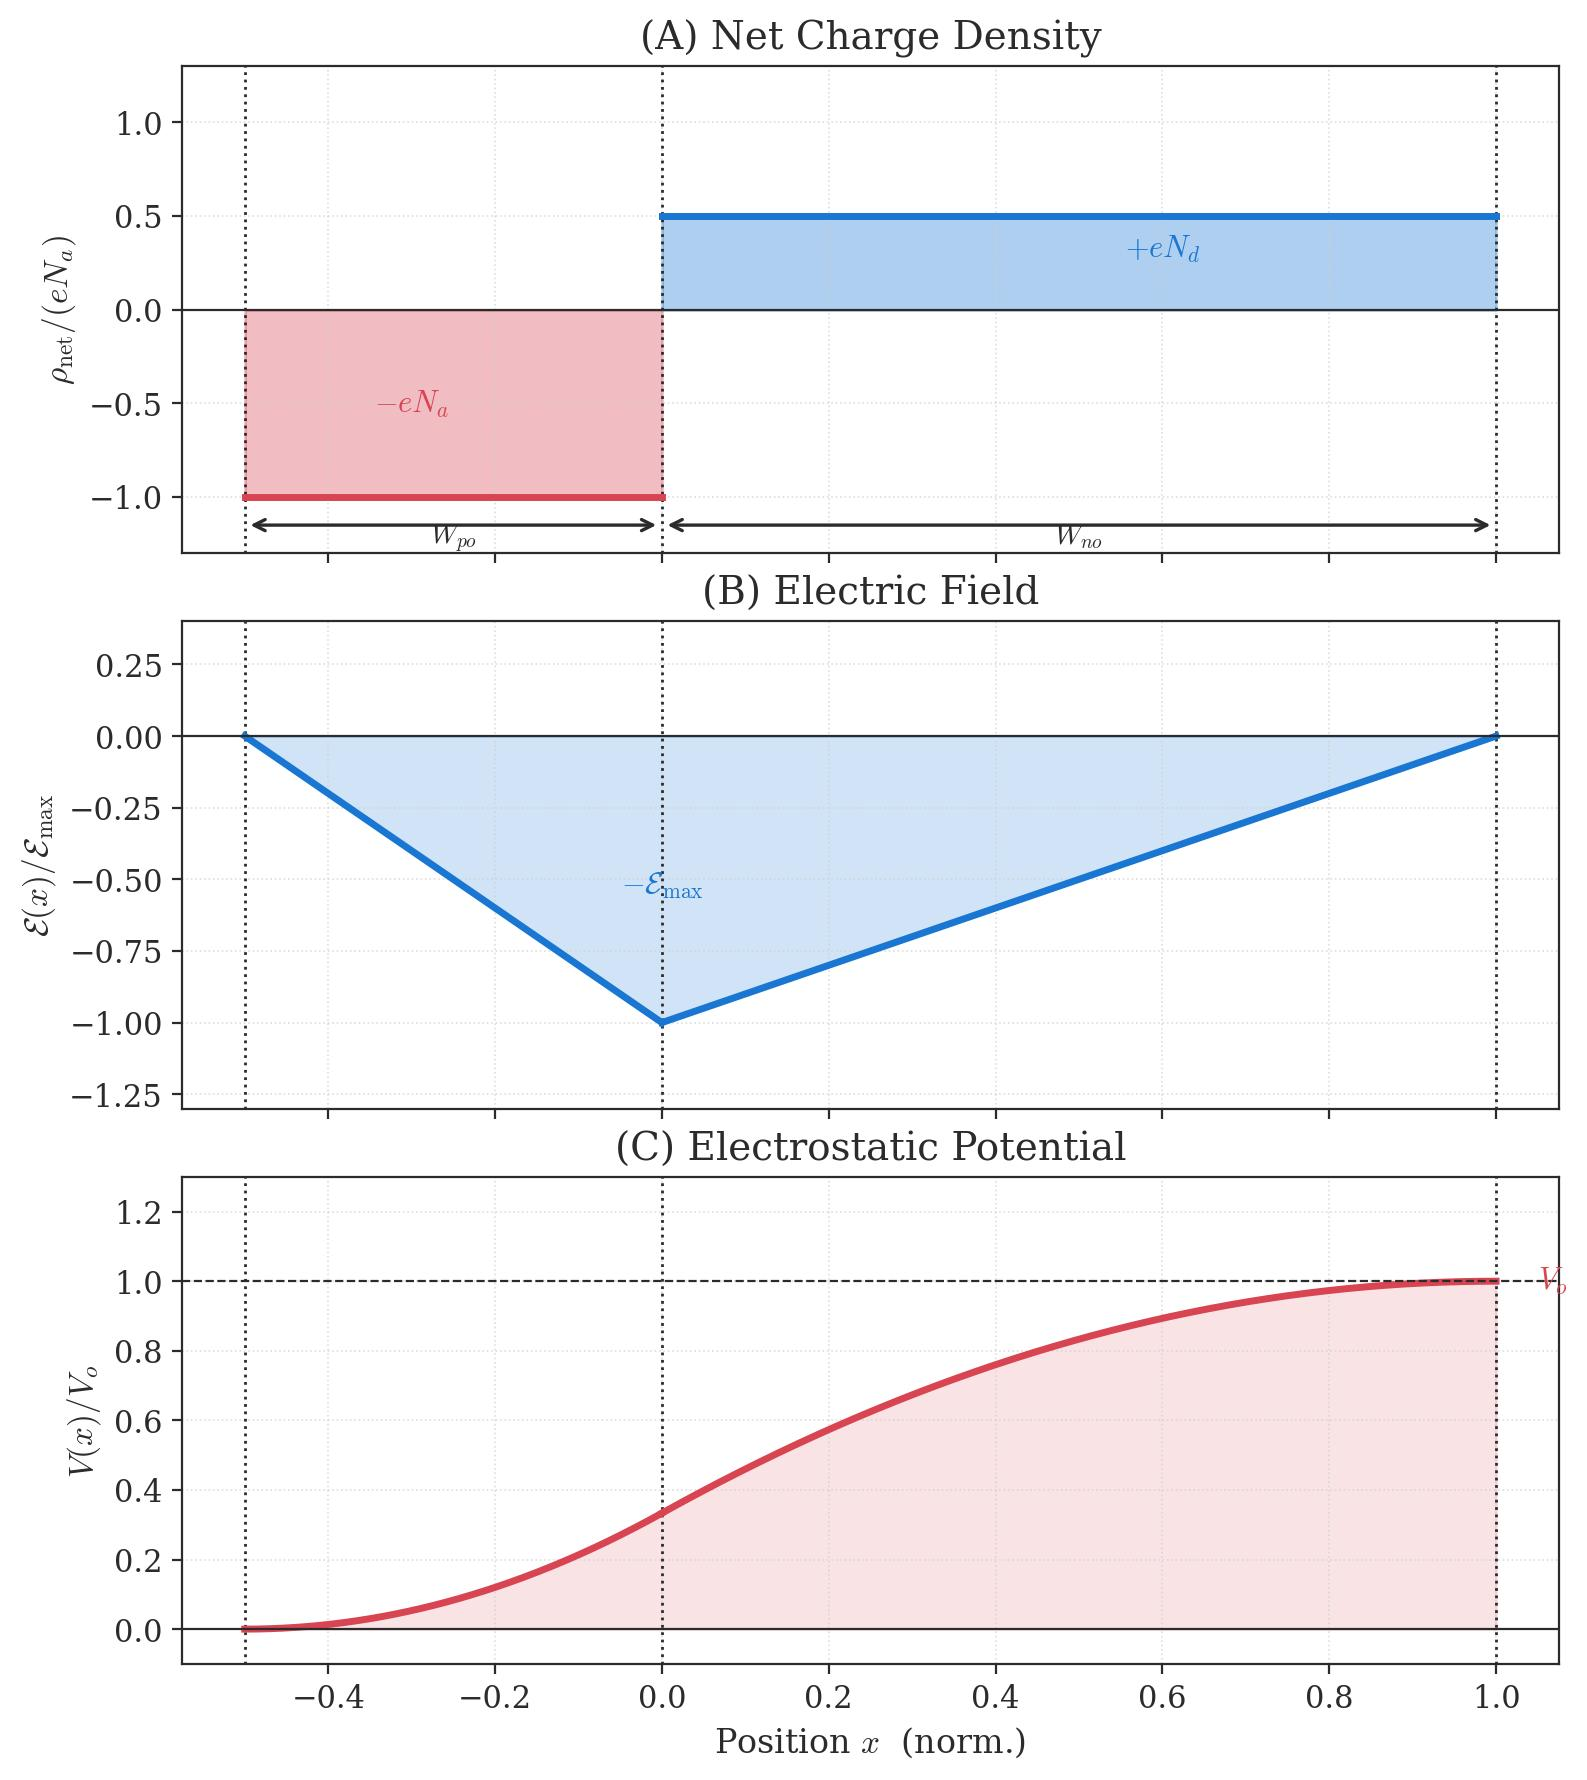
\includegraphics[width=0.75\textwidth]{Figures/Chapter 6/depletion_profiles.jpg}
    \caption{Depletion Region Profiles: Charge Density, Electric Field, and Potential}
\end{figure}

For a typical GaAs homojunction with $N_a \sim N_d \sim 10^{17}\,\text{cm}^{-3}$, the total depletion width $W_0$ is of order tens of nanometres — far narrower than the micron-scale diffusion length $L_D = \sqrt{D\tau}$ over which injected minority carriers ultimately spread. This size mismatch is the root cause of the homojunction's poor efficiency, which we will return to shortly.

% ------------------------------------------------------------------
\section{The Homojunction Under Forward Bias}
% ------------------------------------------------------------------

\subsection{Quasi-Fermi Levels and Minority Carrier Injection}

Applying a forward voltage $V$ lowers the built-in barrier from $eV_0$ to $e(V_0 - V)$, allowing majority carriers to flood across the junction. The device is now far from thermal equilibrium: the electron and hole populations are both elevated simultaneously in the depletion region. As established in the previous chapter, we describe this non-equilibrium state with two separate quasi-Fermi levels $E_{fn}$ and $E_{fp}$, one for each carrier species.

The fundamental physical justification for using quasi-Fermi levels is a massive timescale separation between two distinct processes.

In thermodynamics, the Fermi-Dirac distribution strictly applies only to systems in perfect thermal equilibrium. However, a forward-biased p-n junction is actively driven out of equilibrium as carriers are continuously injected and forced to recombine. By all rights, equilibrium statistics should break down.

We are saved by the fact that carriers undergo two processes with vastly different timescales:
\begin{enumerate}
    \item \textbf{Thermalisation (Fast):} When electrons are injected into the conduction band, they scatter off each other and the crystal lattice, rapidly sharing their energy. This intra-band thermalisation process occurs on a timescale of roughly $\sim 10^{-13}\,\text{s}$ (100 femtoseconds).
    \item \textbf{Recombination (Slow):} The inter-band process of an electron dropping into the valence band to annihilate a hole and emit a photon takes roughly $\sim 10^{-9}\,\text{s}$ (1 nanosecond).
\end{enumerate}

Because the intra-band thermalisation process is $10,000$ times faster than the inter-band recombination process, the electrons reach a state of internal thermal equilibrium \emph{with themselves} long before they recombine. The holes in the valence band independently do the exact same thing. 

Therefore, even though the electron and hole populations are completely out of equilibrium \emph{with each other}, each population is internally well-behaved. This allows us to mathematically treat them as two separate, isolated populations, each governed by its own Fermi-Dirac distribution and its own quasi-Fermi level ($E_{fn}$ for electrons and $E_{fp}$ for holes).

The carrier populations injected across the depletion boundaries under a forward bias voltage $V$ are governed by the Shockley boundary conditions (the law of the junction). At the edge of the depletion region on the p-side, the total electron concentration increases to:
\begin{equation*}
    n_p(0) = n_{p0} \exp\!\left(\frac{qV}{k_B T}\right)
\end{equation*}
where $n_{p0}$ is the equilibrium minority electron concentration. The excess carrier density at the depletion edge is therefore:
\begin{equation*}
    \Delta n_p(0) = n_p(0) - n_{p0} = n_{p0} \left[\exp\!\left(\frac{qV}{k_B T}\right) - 1\right]
\end{equation*}
In the neutral p-bulk, these injected electrons diffuse and recombine, satisfying the 1D steady-state minority carrier diffusion equation:
\begin{equation*}
    D_e \frac{d^2 \Delta n_p}{dx^2} - \frac{\Delta n_p}{\tau_e} = 0
\end{equation*}
Solving this differential equation with boundary conditions $\Delta n_p(0)$ at the depletion edge and $\Delta n_p(\infty) = 0$ yields the spatial decay profile of the injected minority carriers:
\begin{equation*}
    \Delta n_p(x) = \Delta n_p(0) \exp\!\left(-\frac{x}{L_e}\right) = n_{p0} \left[\exp\!\left(\frac{qV}{k_B T}\right) - 1\right] \exp\!\left(-\frac{x}{L_e}\right)
\end{equation*}
where $L_e = \sqrt{D_e \tau_e}$ is the minority electron diffusion length. At the depletion boundary ($x=0$), the fractional excess carrier concentration is:
\begin{equation*}
    \frac{\Delta n_p(0)}{n_{p0}} = \exp\!\left(\frac{qV}{k_BT}\right) - 1
\end{equation*}

This exponential dependence on voltage is the classic diode equation — a small increase in forward bias produces an enormous increase in injected minority carriers. At a forward bias of $V \approx 1\,\text{V}$ for GaAs (where $E_g \approx 1.42\,\text{eV}$), the quasi-Fermi level separation is $E_{fn} - E_{fp} = eV \approx E_g$, and the Bernard-Duraffourg condition is on the verge of being met.

\begin{figure}[H]
    \centering
    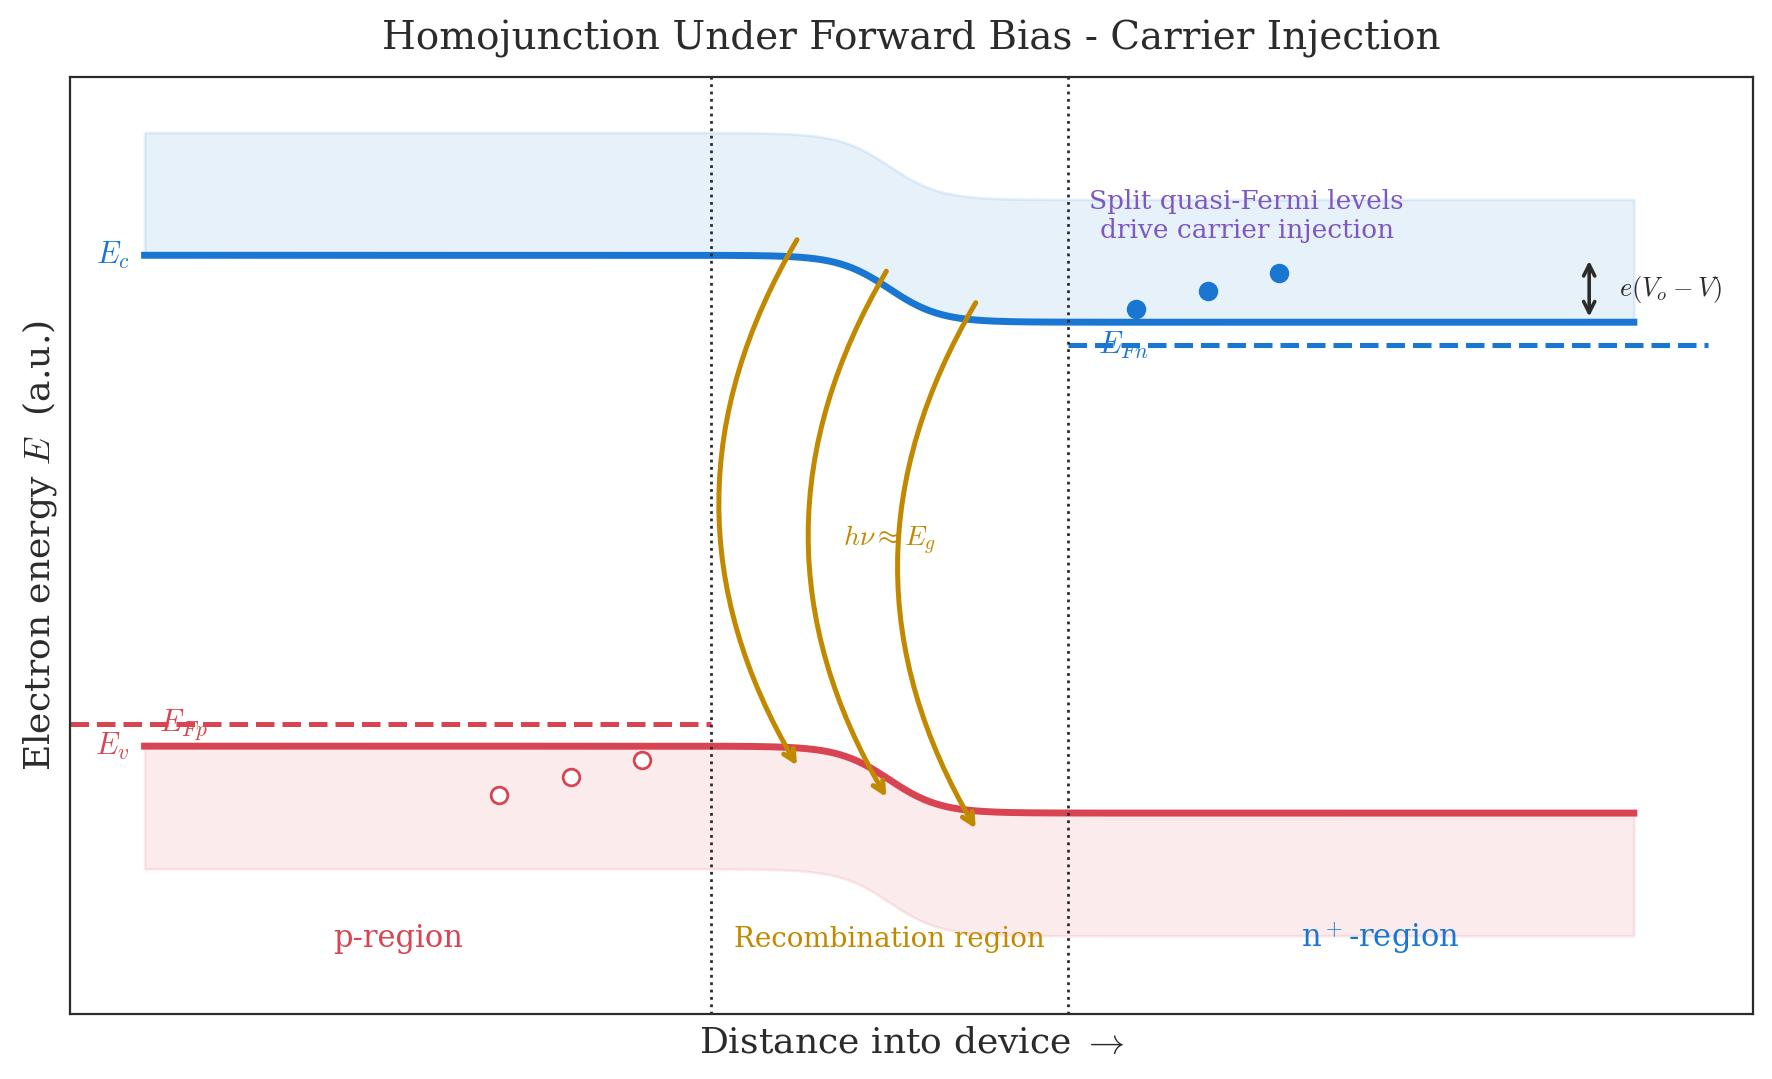
\includegraphics[width=0.65\textwidth]{Figures/Chapter 6/homojunction_forward_bias.jpg}
    \caption{Homojunction Band Diagram Under Forward Bias}
\end{figure}

% ------------------------------------------------------------------
\section{Optical Gain in Semiconductors}
% ------------------------------------------------------------------

\subsection{From Atomic Gain to Band Gain}

The gain coefficient for a collection of two-level atoms has the form $\gamma = \sigma(N_2 - N_1)$, where $\sigma$ is the stimulated emission cross-section and $(N_2 - N_1)$ is the population inversion. That result was derived by treating the active medium as a collection of identical, isolated resonators each with two sharp energy levels. The same physical logic carries over to a semiconductor, but we must now account for the fundamental difference: instead of two sharp levels, we have continuous bands filled with a distribution of states, each pair at a different energy, each with its own occupation probability.

\begin{figure}[H]
    \centering
    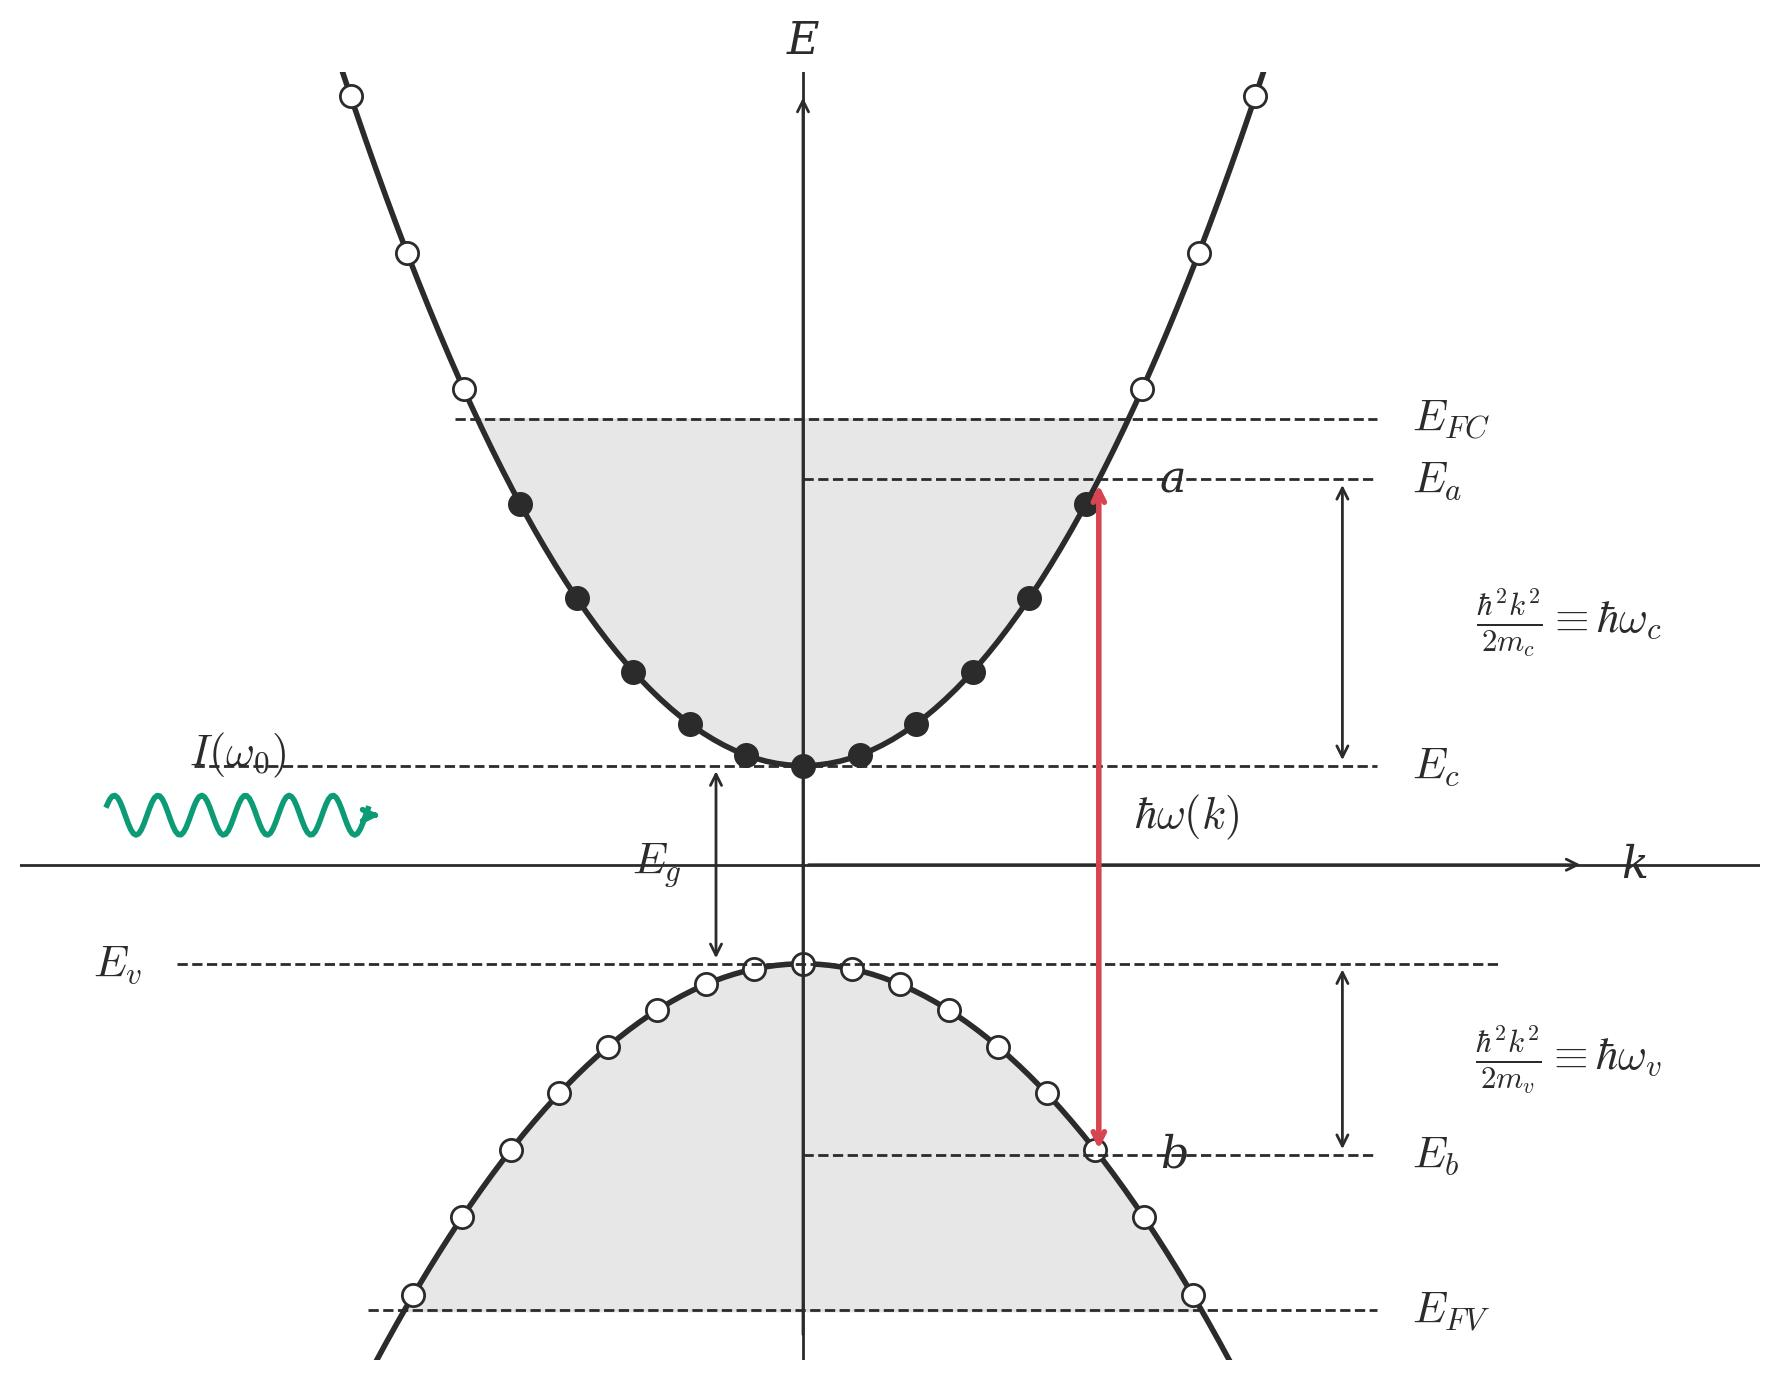
\includegraphics[width=0.65\textwidth]{Figures/Chapter 6/band_gain_ek.jpg}
    \caption{Energy-momentum ($E-k$) diagram illustrating an optical transition between the conduction and valence bands. The transition must conserve momentum, resulting in a vertical arrow.}
\end{figure}

For a photon of energy $h\nu$ to stimulate an optical transition, it must interact with a pair of states: an electron at energy $E_a$ in the conduction band and an empty state (a hole) at energy $E_b$ in the valence band, satisfying energy conservation:
\begin{equation*}
    E_a - E_b = h\nu
\end{equation*}

Near the band edges, both bands are parabolic. The electron energy in the conduction band is:
\begin{equation*}
    E_a = E_c + \frac{(\hbar k)^2}{2m_c^*}
\end{equation*}
and the hole energy (measured from the valence band edge) is:
\begin{equation*}
    E_b = E_v - \frac{(\hbar k)^2}{2m_v^*}
\end{equation*}
where $m_c^*$ and $m_v^*$ are the effective masses in the conduction and valence bands. Subtracting:
\begin{equation*}
    E_a - E_b = (E_c - E_v) + \frac{(\hbar k)^2}{2m_c^*} + \frac{(\hbar k)^2}{2m_v^*} = E_g + \frac{(\hbar k)^2}{2m_r}
\end{equation*}
where we have defined the \textbf{reduced mass} $m_r$:
\begin{keyresult}
    \begin{equation}
        \frac{1}{m_r} = \frac{1}{m_c^*} + \frac{1}{m_v^*}
    \end{equation}
\end{keyresult}

This reduced mass is not merely a mathematical grouping—it represents a profound physical mechanism. Because a photon carries negligible momentum, an optical transition must be strictly \textbf{vertical} on the $E-k$ diagram ($k_e \approx k_h$). This means the electron and hole cannot be treated as independent particles; they are rigidly coupled by momentum conservation and must share the exact same wavevector $k$. 

Consequently, the photon must provide enough energy to overcome the inertia of \textit{both} bands simultaneously. The reduced mass $m_r$ allows us to map this coupled two-particle system onto a \textbf{single fictitious particle}. Instead of tracking two particles in two bands, $m_r$ represents the effective inertia of the transition itself.

By conservation of energy, the photon must provide exactly the energy required to bridge this specific gap. Therefore, we set the photon energy $h\nu$ equal to the total transition energy:
\begin{equation*}
    h\nu = E_g + \frac{\hbar^2 k^2}{2m_r}
\end{equation*}
we can rearrange this to isolate the shared kinetic energy term:
\begin{equation*}
    \frac{\hbar^2 k^2}{2} = m_r(h\nu - E_g)
\end{equation*}

By substituting this isolated kinetic energy term back into the original parabolic equation for the conduction band electron, we can exactly determine how the excess energy partitions:
\begin{equation*}
    E_a = E_c + \frac{1}{m_c^*}\left[\frac{\hbar^2 k^2}{2}\right] \Rightarrow E_a = E_c + \frac{1}{m_c^*}\left[m_r(h\nu - E_g)\right] \Rightarrow E_a = E_c + \frac{m_r}{m_c^*}(h\nu - E_g)
\end{equation*}

Applying the exact same substitution for the corresponding hole state in the valence band:
\begin{equation*}
    E_b = E_v - \frac{1}{m_v^*}\left[\frac{\hbar^2 k^2}{2}\right] \Rightarrow E_b = E_v - \frac{1}{m_v^*}\left[m_r(h\nu - E_g)\right] \Rightarrow E_b = E_v - \frac{m_r}{m_v^*}(h\nu - E_g)
\end{equation*}

Notice the mechanism of energy partitioning: if the conduction band is very "heavy" (large $m_c^*$) and the valence band is very "light" (small $m_v^*$), the lighter particle will absorb the vast majority of the photon's kinetic energy. Because the vertical transition requires a specific $k$ to satisfy momentum conservation, a given photon energy $h\nu$ uniquely maps to exactly one paired state $(E_a, E_b)$.

\subsection{The Joint Density of States}

To calculate the optical gain or absorption spectrum, we need to know how many valid transition pathways exist at a given photon energy $h\nu$. 

It is tempting to simply use the standard single-band density of states ($\rho_c(E)$ or $\rho_v(E)$) for this. However, the normal DOS only tracks the number of "available seats" in one band at a time. Because an optical transition is a strictly \emph{vertical} process on the $E-k$ diagram ($k_a = k_b$), finding an electron at energy $E_a$ in the conduction band is useless if there is no corresponding empty state (hole) at $E_b$ directly below it. 

Therefore, we must count the \emph{simultaneous availability} of coupled pairs of states. We define the \textbf{joint density of states} $\rho(\nu)$ as the number of valid transition pairs per unit volume per unit frequency interval. It is called "joint" because it mathematically fuses the two bands together—using the reduced mass $m_r$ to represent the transition as a single fictitious particle with a unified inertia.

The mathematical derivation of $\rho(\nu)$ mirrors the single-band density of states exactly, with $m_r$ replacing the single-band effective mass. We start from the fact that a photon of energy $h\nu$ can only interact with pairs of states $(E_a, E_b)$ satisfying both energy conservation ($E_a - E_b = h\nu$) and momentum conservation ($k_a = k_b$, since the photon carries negligible momentum). These two constraints rigidly fix a unique value of crystal momentum:
\begin{equation*}
    h\nu = E_g + \frac{\hbar^2 k^2}{2m_r} \implies k = \sqrt{\frac{2m_r(h\nu - E_g)}{\hbar^2}}
\end{equation*}

The number of such pairs in a shell of k-space between $k$ and $k + dk$ (with spin degeneracy factor 2, per unit volume) is:
\begin{equation*}
    d(\text{pairs}) = 2\cdot\frac{4\pi k^2\,dk}{(2\pi)^3} = \frac{k^2\,dk}{\pi^2}
\end{equation*}

Differentiating the dispersion relation to convert $dk$ to $d(h\nu)$:
\begin{equation*}
    \frac{d(h\nu)}{dk} = \frac{\hbar^2 k}{m_r} \implies dk = \frac{m_r}{\hbar^2 k}\,d(h\nu)
\end{equation*}

Substituting $k$ and $dk$ and defining $\rho(\nu) = d(\text{pairs})/d\nu$:
\begin{equation*}
    \rho(\nu)\,d\nu = \frac{k^2}{\pi^2}\cdot\frac{m_r}{\hbar^2 k}\cdot\frac{d(h\nu)}{h}
    = \frac{m_r\,k}{\pi^2\hbar^2 h}\,d(h\nu)
\end{equation*}

Substituting $k = \sqrt{2m_r(h\nu - E_g)}/\hbar$:
\begin{equation*}
    \rho(\nu) = \frac{m_r}{\pi^2\hbar^2 h}\cdot\frac{\sqrt{2m_r(h\nu-E_g)}}{\hbar}
    = \frac{m_r\sqrt{2m_r}}{\pi^2\hbar^3 h}\sqrt{h\nu - E_g}
\end{equation*}

Writing $\hbar = h/(2\pi)$ so that $\hbar^3 = h^3/(8\pi^3)$:
\begin{equation*}
    \rho(\nu) = \frac{m_r\sqrt{2m_r}}{\pi^2\cdot\frac{h^3}{8\pi^3}\cdot h}\sqrt{h\nu - E_g}
    = \frac{8\pi^3 m_r\sqrt{2m_r}}{\pi^2 h^4}\sqrt{h\nu - E_g}
    = \frac{8\pi m_r\sqrt{2m_r}}{h^4}\sqrt{h\nu - E_g}
\end{equation*}

This can be written more compactly by noting that $m_r\sqrt{2m_r} = \sqrt{(2m_r)^3}/2$:
\begin{keyresult}
    \begin{equation}
        \rho(\nu) = \frac{\sqrt{(2m_r)^3}}{\pi^2\hbar^3}\sqrt{h\nu - E_g}, \qquad h\nu \geq E_g
    \end{equation}
\end{keyresult}

This square-root form is identical in structure to the single-band density of states — the joint DOS is zero below the bandgap (no transitions can occur), and grows as a square root above it. The effective mass that controls the curvature is $m_r$, the reduced mass that accounts for both the curvature of the conduction band and the curvature of the valence band simultaneously.

\begin{figure}[H]
    \centering
    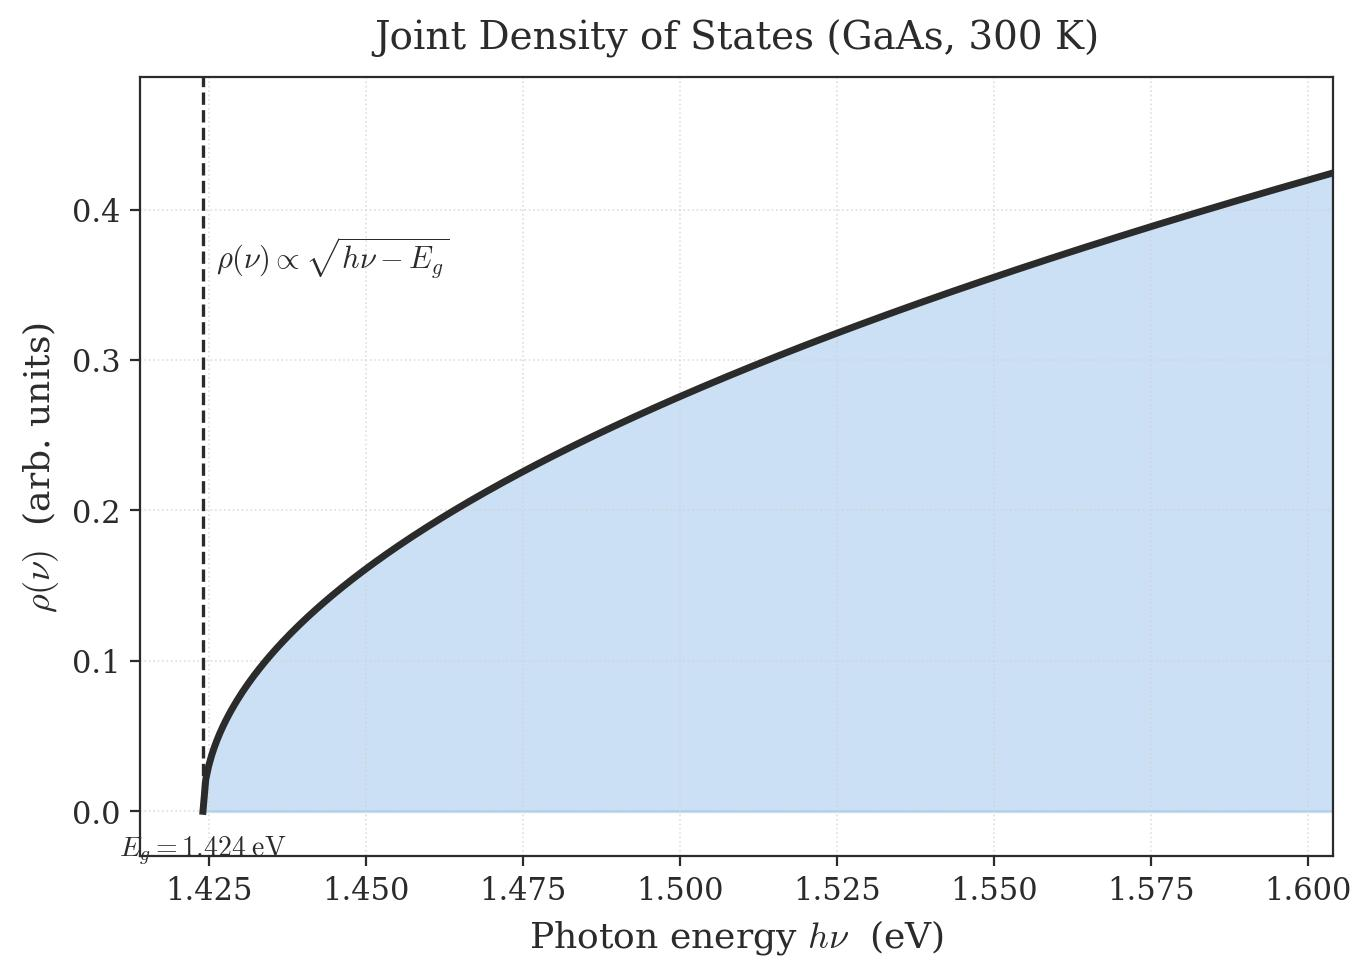
\includegraphics[width=0.65\textwidth]{Figures/Chapter 6/joint_dos.jpg}
    \caption{Joint Density of States $\rho(\nu)$}
\end{figure}

\subsection{The Full Gain Formula}

Now we are ready to write down the net gain coefficient $\gamma(\nu)$. Recall that gain specifically measures the coherent amplification of an electromagnetic wave traveling through the material ($\frac{dI}{dz} = \gamma I$). Therefore, the net gain depends entirely on a tug-of-war between two processes that interact directly with that specific wave:
\begin{enumerate}
    \item \textbf{Stimulated Emission (+):} Creates a perfect clone of an incident photon (same phase, frequency, and direction), adding constructively to amplify the wave.
    \item \textbf{Absorption (-):} Removes a photon from the incident wave, attenuating it.
\end{enumerate}

Notably, \textbf{spontaneous emission is explicitly excluded} from the gain definition. Even though a massive amount of spontaneous emission occurs (it's what makes the device glow), these photons are emitted with random phases and in random directions. They do not add constructively to amplify the traveling coherent wave; they simply exit the device or act as incoherent background noise. Therefore, at photon energy $h\nu$, the net gain is solely the stimulated emission rate minus the absorption rate, summed over all transition pairs.

The probability of finding an electron in state $E_a$ (needed for stimulated emission) is $f_c(E_a)$ — the Fermi-Dirac distribution evaluated with the electron quasi-Fermi level $E_{fc}$. The probability of finding the corresponding state $E_b$ empty (i.e., occupied by a hole, needed for emission) is $[1 - f_v(E_b)]$, where $f_v(E_b)$ uses the hole quasi-Fermi level $E_{fv}$.

The net gain coefficient is proportional to the joint density of states, weighted by the net inversion factor — the probability of stimulated emission minus the probability of absorption. To derive the exact prefactor, we use Einstein's thermodynamic theory of radiative transitions adapted to a semiconductor.

For a mode with spectral energy density $u(\nu)$ and refractive index $n$, the group velocity is $v_g = c/n$. The transition rates per unit volume per unit frequency interval are:
\begin{align*}
    r_{sp}(\nu) &= A_{21}\,\rho(\nu)\,f_c(E_a)\!\left[1 - f_v(E_b)\right] \\
    r_{st}(\nu) &= B_{21}\,u(\nu)\,\rho(\nu)\,f_c(E_a)\!\left[1 - f_v(E_b)\right] \\
    r_{abs}(\nu) &= B_{12}\,u(\nu)\,\rho(\nu)\,f_v(E_b)\!\left[1 - f_c(E_a)\right]
\end{align*}
where $A_{21}$, $B_{21}$, and $B_{12}$ are the Einstein coefficients. Symmetries demand $B_{21} = B_{12}$, and the spontaneous lifetime is $\tau_{sp} = 1/A_{21}$. The relationship between the spontaneous and stimulated emission coefficients in a medium of refractive index $n$ is:
\begin{equation*}
    \frac{A_{21}}{B_{21}} = \frac{8\pi h n^3 \nu^3}{v_g^3} = \frac{8\pi h n^3 \nu^3}{c^3} \implies B_{21} = \frac{c^3}{8\pi h n^3 \nu^3 \tau_{sp}}
\end{equation*}
The net rate of stimulated transition events per unit volume per unit frequency is:
\begin{align*}
    r_{net}(\nu) &= r_{st}(\nu) - r_{abs}(\nu) \\
    &= B_{21}\,u(\nu)\,\rho(\nu)\,\left( f_c(E_a)\!\left[1 - f_v(E_b)\right] - f_v(E_b)\!\left[1 - f_c(E_a)\right] \right) \\
    &= B_{21}\,u(\nu)\,\rho(\nu)\,\left[f_c(E_a) - f_v(E_b)\right]
\end{align*}
The spectral energy density is related to the spectral intensity $I(\nu)$ of the wave by $u(\nu) = I(\nu)/v_g = n I(\nu)/c$. Substituting $B_{21}$ and $u(\nu)$ gives:
\begin{equation*}
    r_{net}(\nu) = \left(\frac{c^3}{8\pi h n^3 \nu^3 \tau_{sp}}\right) \left(\frac{n I(\nu)}{c}\right) \rho(\nu) \left[f_c(E_a) - f_v(E_b)\right] = \frac{c^2 I(\nu)}{8\pi h n^2 \nu^3 \tau_{sp}}\,\rho(\nu)\,\left[f_c(E_a) - f_v(E_b)\right]
\end{equation*}
Each net stimulated emission transition generates one photon of energy $h\nu$. By conservation of energy, the spatial growth of intensity along the propagation direction $z$ is:
\begin{equation*}
    \frac{dI(\nu)}{dz} = h\nu \cdot r_{net}(\nu) = \left(\frac{c^2}{8\pi n^2 \nu^2 \tau_{sp}}\,\rho(\nu)\,\left[f_c(E_a) - f_v(E_b)\right]\right) I(\nu)
\end{equation*}
Since the material gain coefficient $\gamma(\nu)$ is defined by $\frac{dI(\nu)}{dz} = \gamma(\nu) I(\nu)$, we identify the gain coefficient exactly. By explicitly substituting the joint density of states $\rho(\nu)$ and the expanded Fermi-Dirac distributions for the inversion factor $[f_c(E_a) - f_v(E_b)]$, we obtain the full, expanded gain formula:
\begin{keyresult}
    \begin{equation}
        \gamma(\nu) = \frac{c^2}{8\pi n^2\nu^2\,\tau_{sp}} \frac{\sqrt{(2m_r)^3}}{\pi^2\hbar^3}\sqrt{h\nu - E_g} \left[ \frac{1}{1+\exp\!\left(\dfrac{E_a - E_{fc}}{k_BT}\right)} - \frac{1}{1+\exp\!\left(\dfrac{E_b - E_{fv}}{k_BT}\right)} \right]
    \end{equation}
\end{keyresult}
Let us break down the anatomy of this equation to understand exactly what each block represents physically:
\begin{itemize}
    \item \textbf{The Scaling Prefactor} $\left( \frac{c^2}{8\pi n^2\nu^2\,\tau_{sp}} \right)$: This term originates from Einstein's thermodynamic theory of radiation. If you recall from earlier chapters, the stimulated emission cross-section for a simple atomic system is $\sigma = \frac{\lambda^2}{8\pi \tau_{sp}} g(\nu)$. Since the wavelength in the material is $\lambda = c / (n\nu)$, this prefactor is literally exactly that: the \textbf{optical cross-section} scaling factor ($\frac{\lambda^2}{8\pi\tau_{sp}}$). It establishes the fundamental ``target size'' or coupling strength between the electromagnetic wave and the material. It is inversely proportional to $\tau_{sp}$ because a material that spontaneously decays rapidly is fundamentally 'wired' to interact more strongly with stimulated radiation.
    \item \textbf{The Transition Pathways} $\left( \frac{\sqrt{(2m_r)^3}}{\pi^2\hbar^3}\sqrt{h\nu - E_g} \right)$: This is the explicit expansion of the Joint Density of States, $\rho(\nu)$. Physically, it counts the sheer number of valid ``routes''—paired states $(E_a, E_b)$ in the crystal—that are legally allowed to participate in the transition because they perfectly satisfy both energy conservation ($E_a - E_b = h\nu$) and momentum conservation. More available routes mean a mathematically higher probability of the transition occurring.
    \item \textbf{The Net Inversion Factor} $\left[ \frac{1}{1+\exp\!\left(\frac{E_a - E_{fc}}{k_BT}\right)} - \frac{1}{1+\exp\!\left(\frac{E_b - E_{fv}}{k_BT}\right)} \right]$: This bracket is the semiconductor equivalent of atomic population inversion $(N_2 - N_1)$. The first fraction is $f_c(E_a)$, the probability that the upper state is full (ready to emit). The second fraction is $f_v(E_b)$, the probability that the lower state is full (ready to absorb). Their difference explicitly represents the tug-of-war between stimulated emission and absorption. If this bracket evaluates to a positive number, the material amplifies light; if negative, it absorbs.
\end{itemize}

It is important to note that this formula calculates the gain for a \textbf{single, specific frequency} $\nu$. If we need to analyze a signal with a broad spectrum, or calculate the total aggregate stimulated emission rate across a \textbf{band of frequencies}, we must mathematically integrate this entire expression over that frequency range.

\begin{figure}[H]
    \centering
    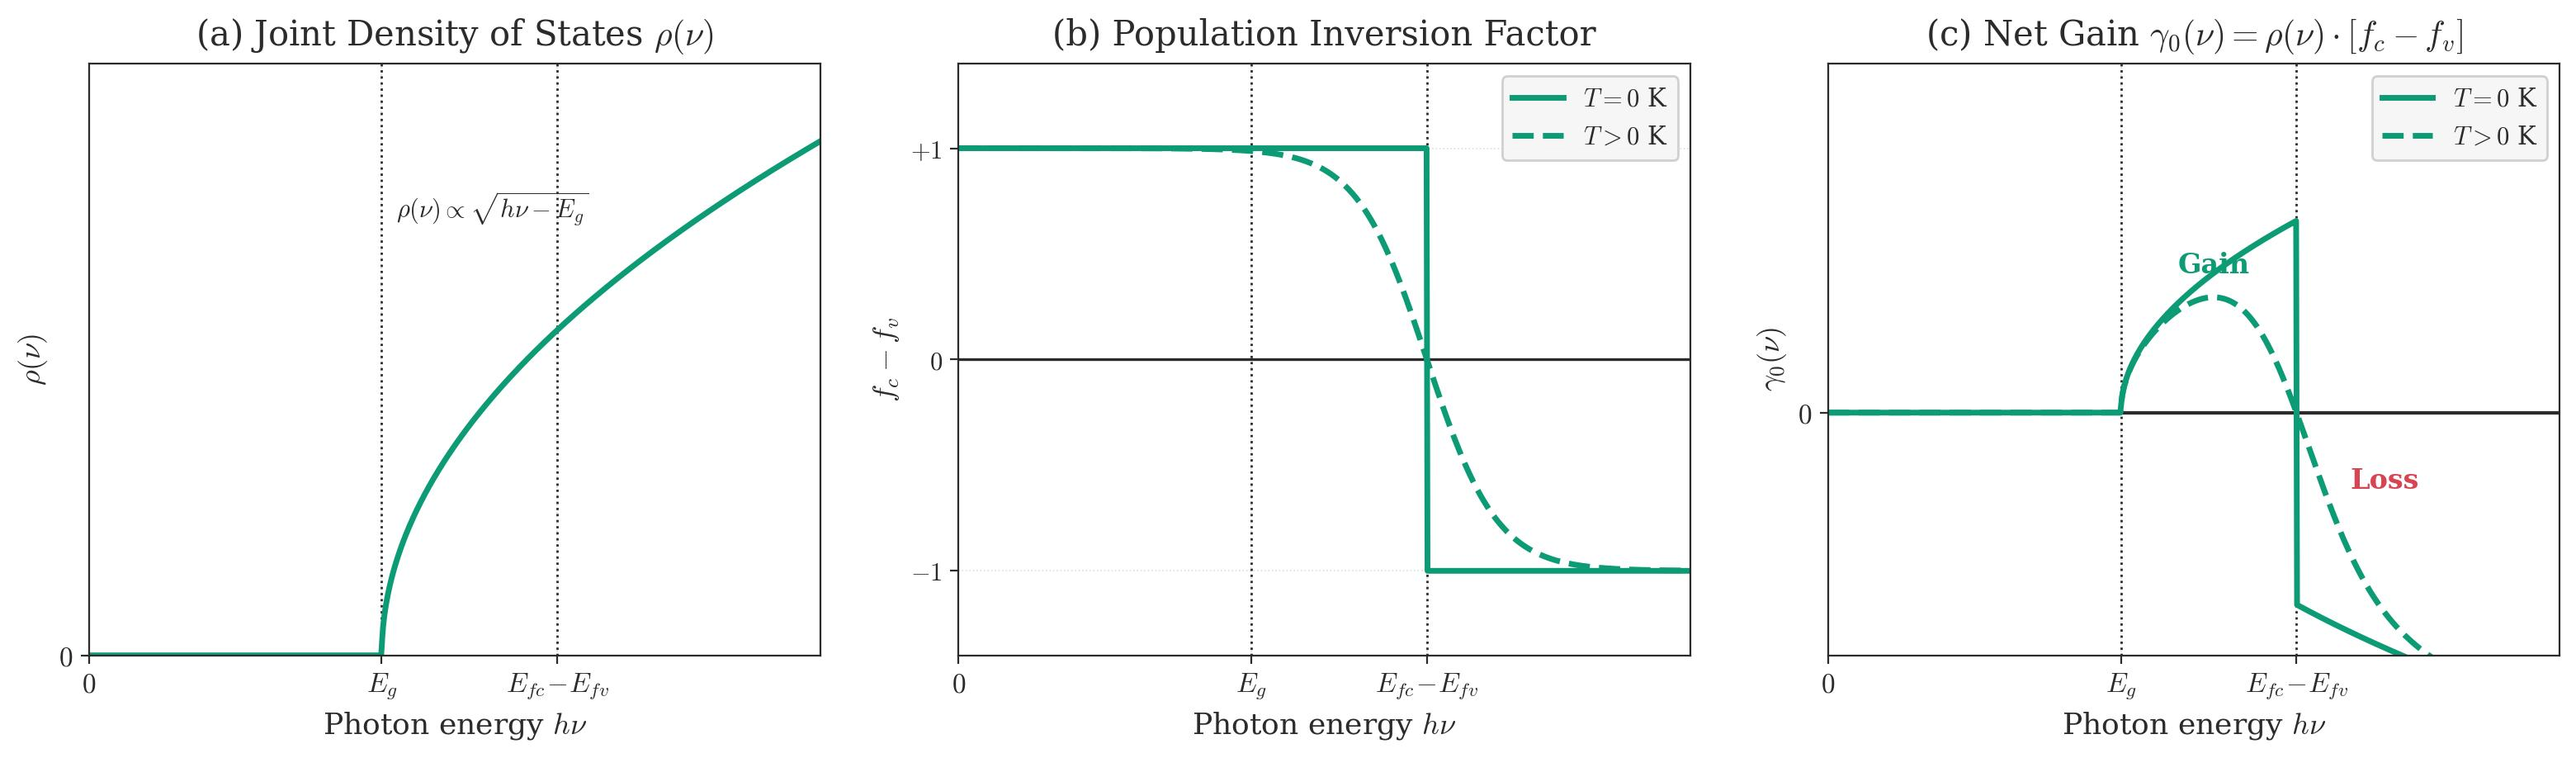
\includegraphics[width=0.95\textwidth]{Figures/Chapter 6/gain_formula_decomposition.jpg}
    \caption{Conceptual Decomposition of the Net Gain Formula $\gamma_0(\nu) = \rho(\nu) \cdot [f_c - f_v]$}
\end{figure}

To see when this material actually amplifies light (i.e., when $\gamma(\nu) > 0$), we simply require the net inversion bracket to be positive:
\begin{equation*}
    \frac{1}{1+\exp\!\left(\frac{E_a - E_{fc}}{k_BT}\right)} > \frac{1}{1+\exp\!\left(\frac{E_b - E_{fv}}{k_BT}\right)}
\end{equation*}

Because the function $1/(1+x)$ strictly decreases as $x$ increases, this inequality holds if and only if the exponent on the left is smaller than the exponent on the right:
\begin{equation*}
    E_a - E_{fc} < E_b - E_{fv}
\end{equation*}

Rearranging the terms to group the electron/hole state energies on one side and the quasi-Fermi levels on the other gives:
\begin{equation*}
    E_a - E_b < E_{fc} - E_{fv}
\end{equation*}

But we already know from fundamental energy conservation that the transition gap $E_a - E_b$ must exactly equal the photon energy $h\nu$. Furthermore, the photon energy must be at least the bandgap $E_g$ for any states to even exist. Substituting $h\nu$ into the inequality yields the final fundamental requirement for optical gain:
\begin{keyresult}
    \begin{equation}
        E_{fc} - E_{fv} > h\nu > E_g
    \end{equation}
\end{keyresult}

This is exactly the \textbf{Bernard-Duraffourg condition}. There are no tricks or external assumptions here: the macroscopic threshold for population inversion drops out as a mathematically rigorous, unavoidable consequence of the Fermi-Dirac statistics inside the gain formula.

\begin{figure}[H]
    \centering
    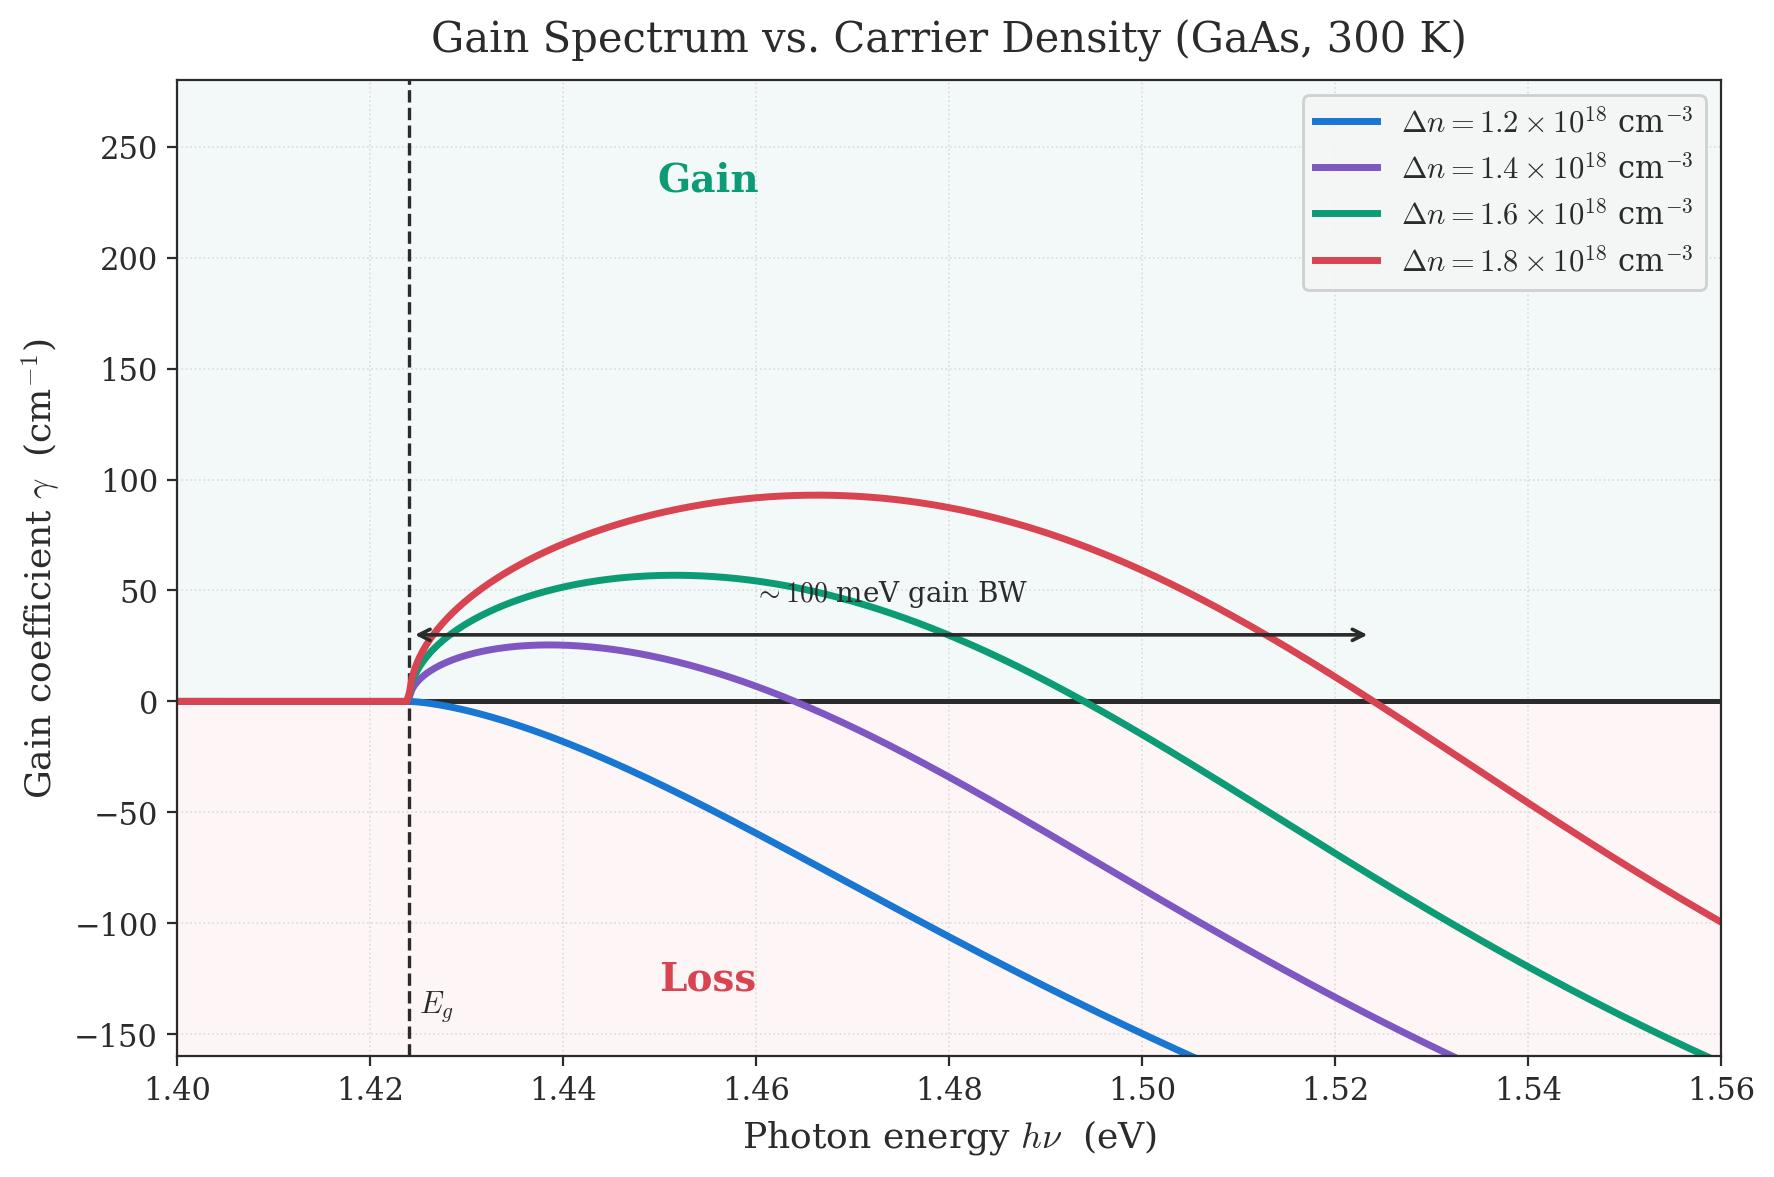
\includegraphics[width=0.65\textwidth]{Figures/Chapter 6/gain_spectrum_carrier_densities.jpg}
    \caption{Gain Spectrum $\gamma(h\nu)$ for Multiple Carrier Densities}
\end{figure}

\subsection{Rates of Optical Transitions}

While we derived the fundamental physics earlier using abstract thermodynamic variables like Einstein coefficients and spectral energy density $u(\nu)$, it is extremely useful for semiconductor device engineering to express the three fundamental optical transition rates ($R_{sp}$, $R_{st}$, and $R_{abs}$) in terms of macroscopic, measurable quantities. 

To do this, we replace the abstract Einstein $A_{21}$ coefficient with the measurable radiative lifetime $\tau_r = 1/A_{21}$. We also replace the field energy density with the incident photon flux. Since the optical intensity $I(\nu)$ is the power per unit area, dividing it by the energy of a single photon $h\nu$ explicitly gives the \textbf{photon flux} $\frac{I(\nu)}{h\nu}$ (the number of photons hitting the material per second per unit area).

The \textbf{spontaneous emission rate} ($R_{sp}$) happens independently of any incident light. It is governed purely by the intrinsic decay rate ($1/\tau_r$), the number of available transition pathways $\rho(\nu)$, and the Fermi-Dirac probability that an electron actually exists in the upper state $f_c(E_a)$ while a hole simultaneously exists in the lower state $[1 - f_v(E_b)]$:
\begin{equation*}
    R_{sp} = \frac{1}{\tau_r}\,\rho(\nu)\,f_c(E_a)\!\left[1 - f_v(E_b)\right]
\end{equation*}

The \textbf{stimulated emission rate} ($R_{st}$) requires the exact same carrier conditions as spontaneous emission, but it is actively driven by the incident photon flux. It is scaled by the fundamental optical cross-section we identified earlier:
\begin{equation*}
    R_{st} = \left( \frac{c^2}{8\pi n^2\nu^2\,\tau_r} \right) \cdot \left[ \frac{I(\nu)}{h\nu} \right] \cdot \rho(\nu) \cdot f_c(E_a)\!\left[1 - f_v(E_b)\right]
\end{equation*}

The \textbf{absorption rate} ($R_{abs}$) is the exact reverse process. It is driven by the exact same incident photon flux and cross-section, but the carrier requirements are inverted: the electron must start in the lower state $f_v(E_b)$ and be promoted to an empty upper state $[1 - f_c(E_a)]$:
\begin{equation*}
    R_{abs} = \left( \frac{c^2}{8\pi n^2\nu^2\,\tau_r} \right) \cdot \left[ \frac{I(\nu)}{h\nu} \right] \cdot \rho(\nu) \cdot f_v(E_b)\!\left[1 - f_c(E_a)\right]
\end{equation*}

By writing the equations in this macroscopic format, it becomes visually obvious that if you subtract absorption from stimulated emission ($R_{st} - R_{abs}$), you factor out the cross-section, the photon flux, and the JDOS, leaving exactly the net inversion bracket $[f_c(E_a) - f_v(E_b)]$ that drives optical gain.

\begin{figure}[H]
    \centering
    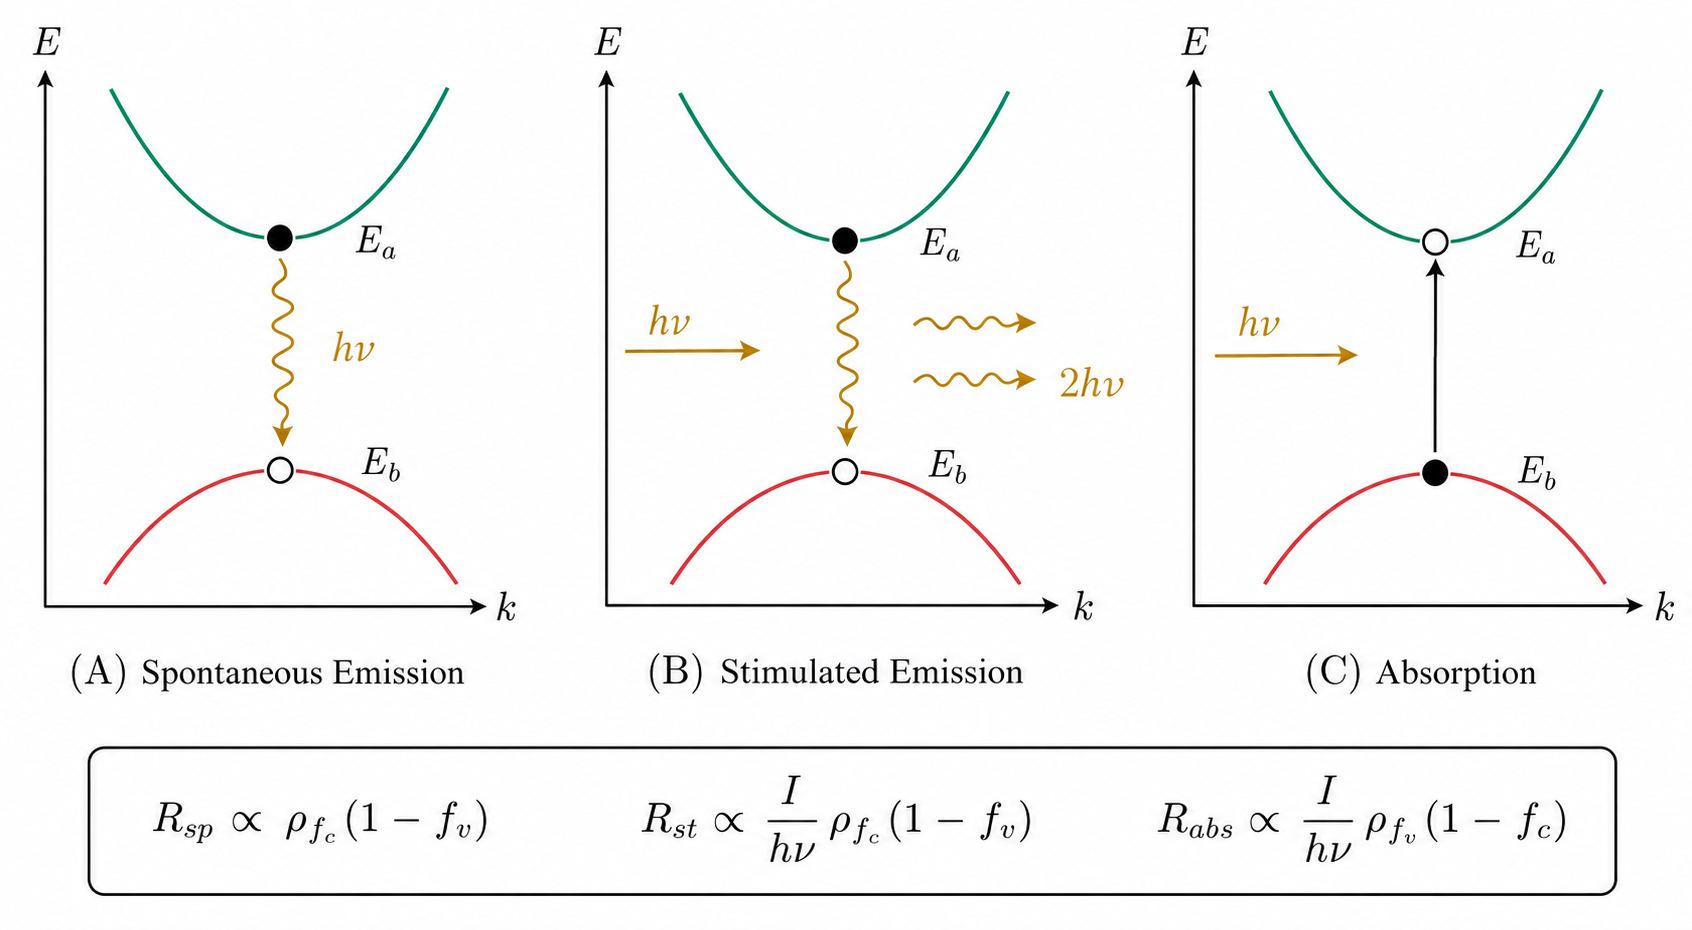
\includegraphics[width=0.65\textwidth]{Figures/Chapter 6/optical_transition_rates_in_a_semiconductor.jpg}
    \caption{Optical Transition Rates in a Semiconductor}
\end{figure}

% ------------------------------------------------------------------
\section{Why the Homojunction Fails in Practice}
% ------------------------------------------------------------------

\subsection{Limitation 1 — Carrier Leakage (The "Thick" Active Region)}

The fundamental problem of a homojunction (a p-n junction made of a single material) is that it lacks physical walls to contain the electrons and holes. When we inject carriers under forward bias, they don't just stay neatly inside the narrow depletion region. Instead, they wander away freely, diffusing deep into the neutral semiconductor bulk on both sides. 

They spread over a distance known as the \textbf{diffusion length} ($L_p = \sqrt{D\tau}$), which is typically around $1\,\mu\text{m}$—orders of magnitude larger than the original junction. Think of this like trying to fill a bucket that has no sides: the carriers just spill out into the bulk crystal. To achieve the high carrier density required for population inversion across this massive, bloated volume, we have to pump an absurdly huge amount of current into the device. The required threshold current density is typically $10^4$--$10^5\,\text{A/cm}^2$, which would melt a practical device at room temperature.

\begin{figure}[H]
    \centering
    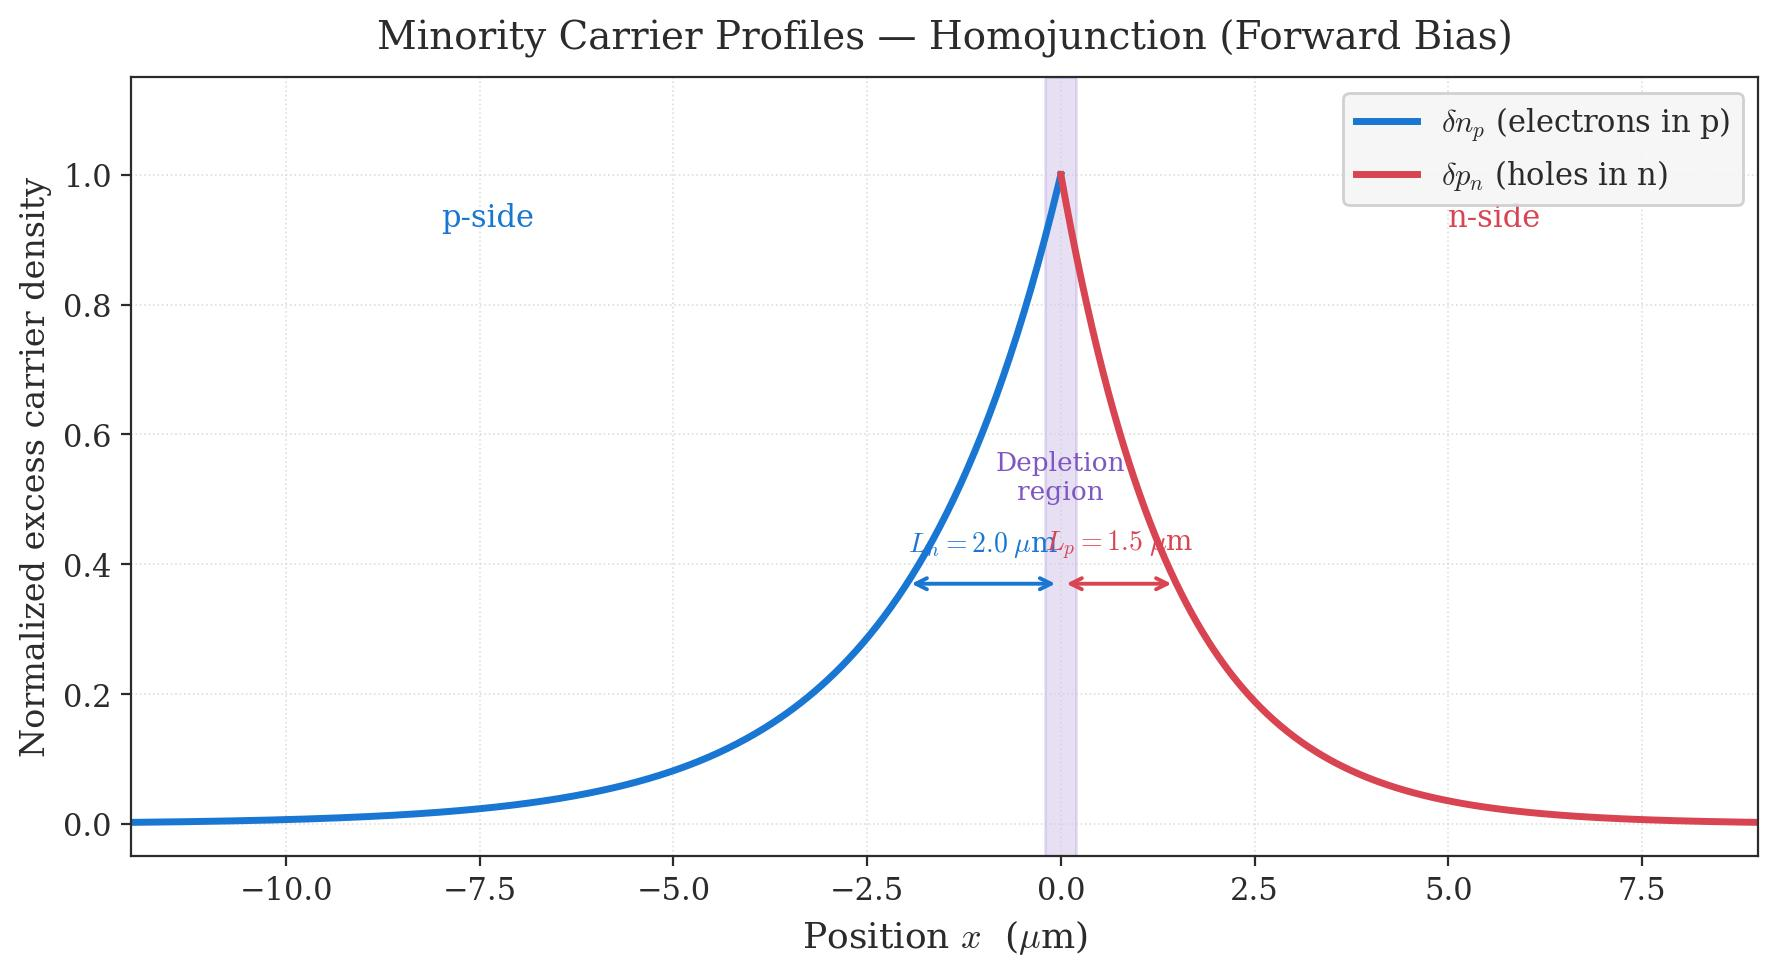
\includegraphics[width=0.65\textwidth]{Figures/Chapter 6/minority_carrier_profile.jpg}
    \caption{Minority Carrier Profile in a Forward-Biased Homojunction}
\end{figure}

\subsection{Limitation 2 — Optical Leakage (Weak Photon Confinement)}

The second problem is that the homojunction also fails to contain the light it produces. Because the entire device is made of the exact same material, the refractive index is virtually identical everywhere. 

Without a difference in refractive index, there is no optical waveguide (no internal reflection) to trap the generated photons near the junction. The optical wave just spreads freely throughout the entire thick crystal. As a result, the vast majority of the photon energy is traveling through the dark, unpumped regions of the semiconductor where it gets absorbed and lost, rather than traveling through the active gain region where it could be amplified. 

In short, a homojunction laser is a leaky bucket for both electrons and photons, making it fundamentally impractical for real-world applications.

% ------------------------------------------------------------------
\section{The Double Heterostructure}
% ------------------------------------------------------------------

\subsection{The Core Idea: Two Confinement Problems, One Solution}

The double heterojunction (DH) laser resolves both limitations simultaneously using a single architectural change: replacing the symmetric homojunction with a three-layer sandwich — a narrow-gap \textbf{active layer} of thickness $d$ (typically $100$--$300\,\text{nm}$) sandwiched between two \textbf{cladding layers} of a wider-gap semiconductor material.

The key property is that the cladding and active materials are different semiconductor compounds, so the structure exploits two material properties simultaneously: the bandgap difference and the refractive index difference.

\subsection{Formation of the Heterojunction Band Diagram}

To understand where the confinement ``walls'' actually come from, it is very instructive to visualize the band diagram in three sequential steps:

\begin{enumerate}
    \item \textbf{Isolated Materials (Before Contact):} When the three layers (P-cladding, active, N-cladding) are completely separated, each material simply has its own flat energy bands, determined by its electron affinity $\chi$ and bandgap $E_g$. The key observation is that the active layer has a \emph{smaller} bandgap and a \emph{different} electron affinity than the two cladding layers — this is the fundamental asymmetry that the entire device exploits.
    \item \textbf{Thermal Equilibrium (Zero Bias):} When the three layers are brought into physical contact, the Fermi levels must equalize across the entire structure (this is the definition of thermal equilibrium). Carriers flow across the interfaces until this is achieved, bending the energy bands. The mismatch in electron affinity and bandgap creates abrupt steps — the band discontinuities $\Delta E_c$ and $\Delta E_v$ — at each interface, forming a quantum well in the active region.
    \item \textbf{Forward Bias (Lasing Condition):} When a voltage $V$ is applied, the Fermi level splits into two quasi-Fermi levels ($E_{Fc}$ and $E_{Fv}$), separated by $qV$. This drives massive injection of electrons and holes into the quantum well. The carriers are trapped inside by the band discontinuity walls, achieving the high carrier density needed for population inversion and stimulated emission.
\end{enumerate}

\begin{figure}[H]
    \centering
    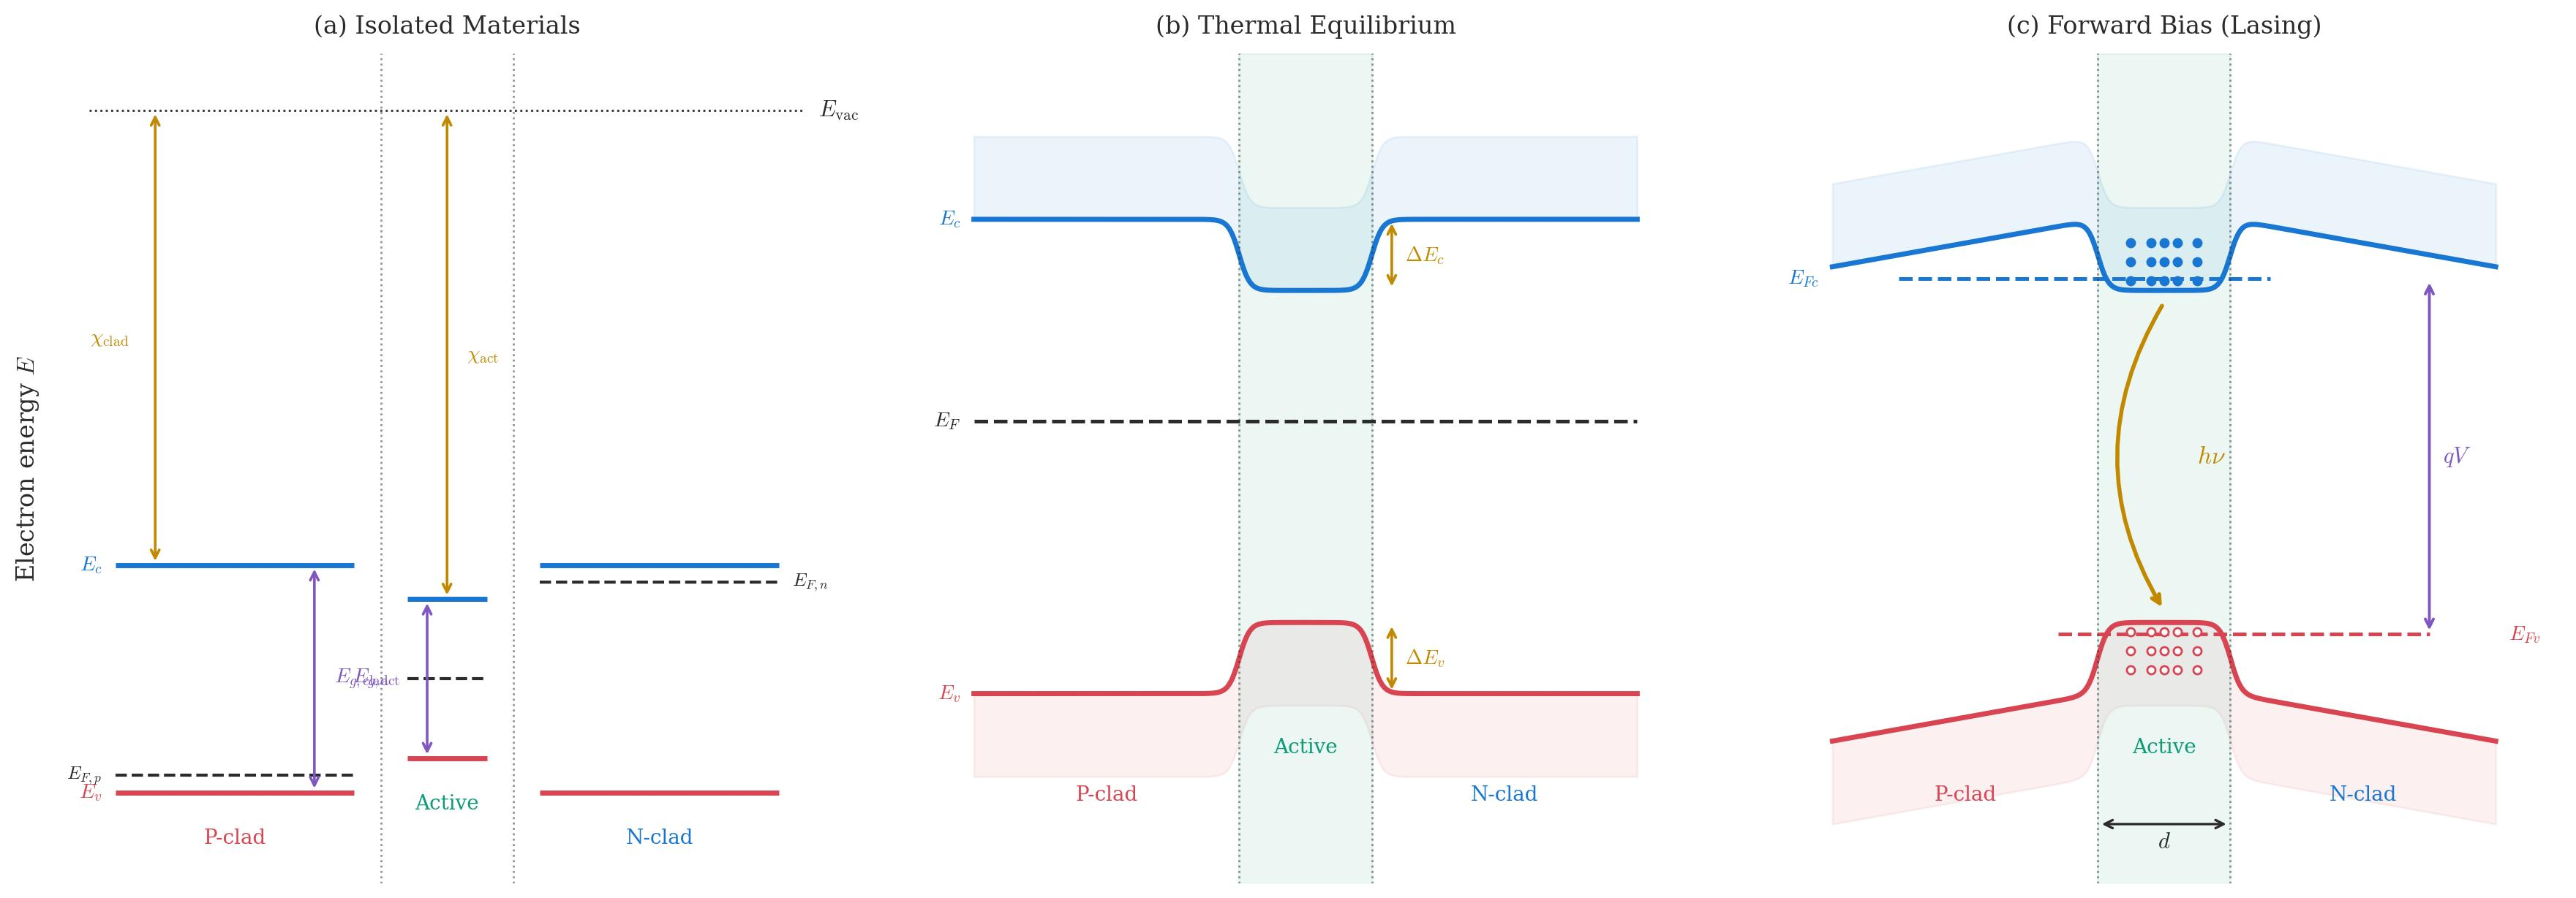
\includegraphics[width=\textwidth]{Figures/Chapter 6/heterojunction_band_formation.jpg}
    \caption{Formation of the Double Heterojunction Band Diagram: (a) Isolated materials aligned to the vacuum level, (b) Thermal equilibrium with flat Fermi level, (c) Forward bias with quasi-Fermi level splitting and carrier injection.}
\end{figure}

\subsection{Carrier Confinement via Band Discontinuities}

Because the active layer has a smaller bandgap than the two surrounding cladding layers, the energy bands do not line up perfectly at the interfaces. Instead, the abrupt change in materials creates a sudden step in the energy levels — a \textbf{band-edge discontinuity} — at both the conduction band ($\Delta E_c$) and the valence band ($\Delta E_v$).

You can think of these discontinuities as physical, energetic walls. The conduction band in the cladding sits much higher than the conduction band in the active layer, creating a steep cliff that electrons cannot easily climb over. Similarly, the valence band in the cladding sits lower, creating a barrier that holes cannot cross.

Because these energy steps are typically much larger than the room-temperature thermal energy ($k_B T \approx 26\text{ meV}$), injected carriers simply do not have the thermal kinetic energy to jump over the walls. 

These discontinuities form \textbf{potential barriers} that physically prevent injected electrons and holes from diffusing out of the active region. The carriers are confined inside the very thin active layer like water trapped in a narrow, high-walled channel. 

This physical confinement is the key breakthrough: the volume that needs to be pumped with current is now entirely restricted to the active layer thickness $d \sim 100\,\text{nm}$, rather than the massive diffusion length $L_p \sim 1\,\mu\text{m}$. Because the ``bucket'' now has walls, the current density required to fill it and achieve population inversion is reduced by a massive factor of $L_p/d \sim 10$--$100$, bringing threshold currents down to highly practical levels ($\sim 1\,\text{kA/cm}^2$ or below).

\begin{figure}[H]
    \centering
    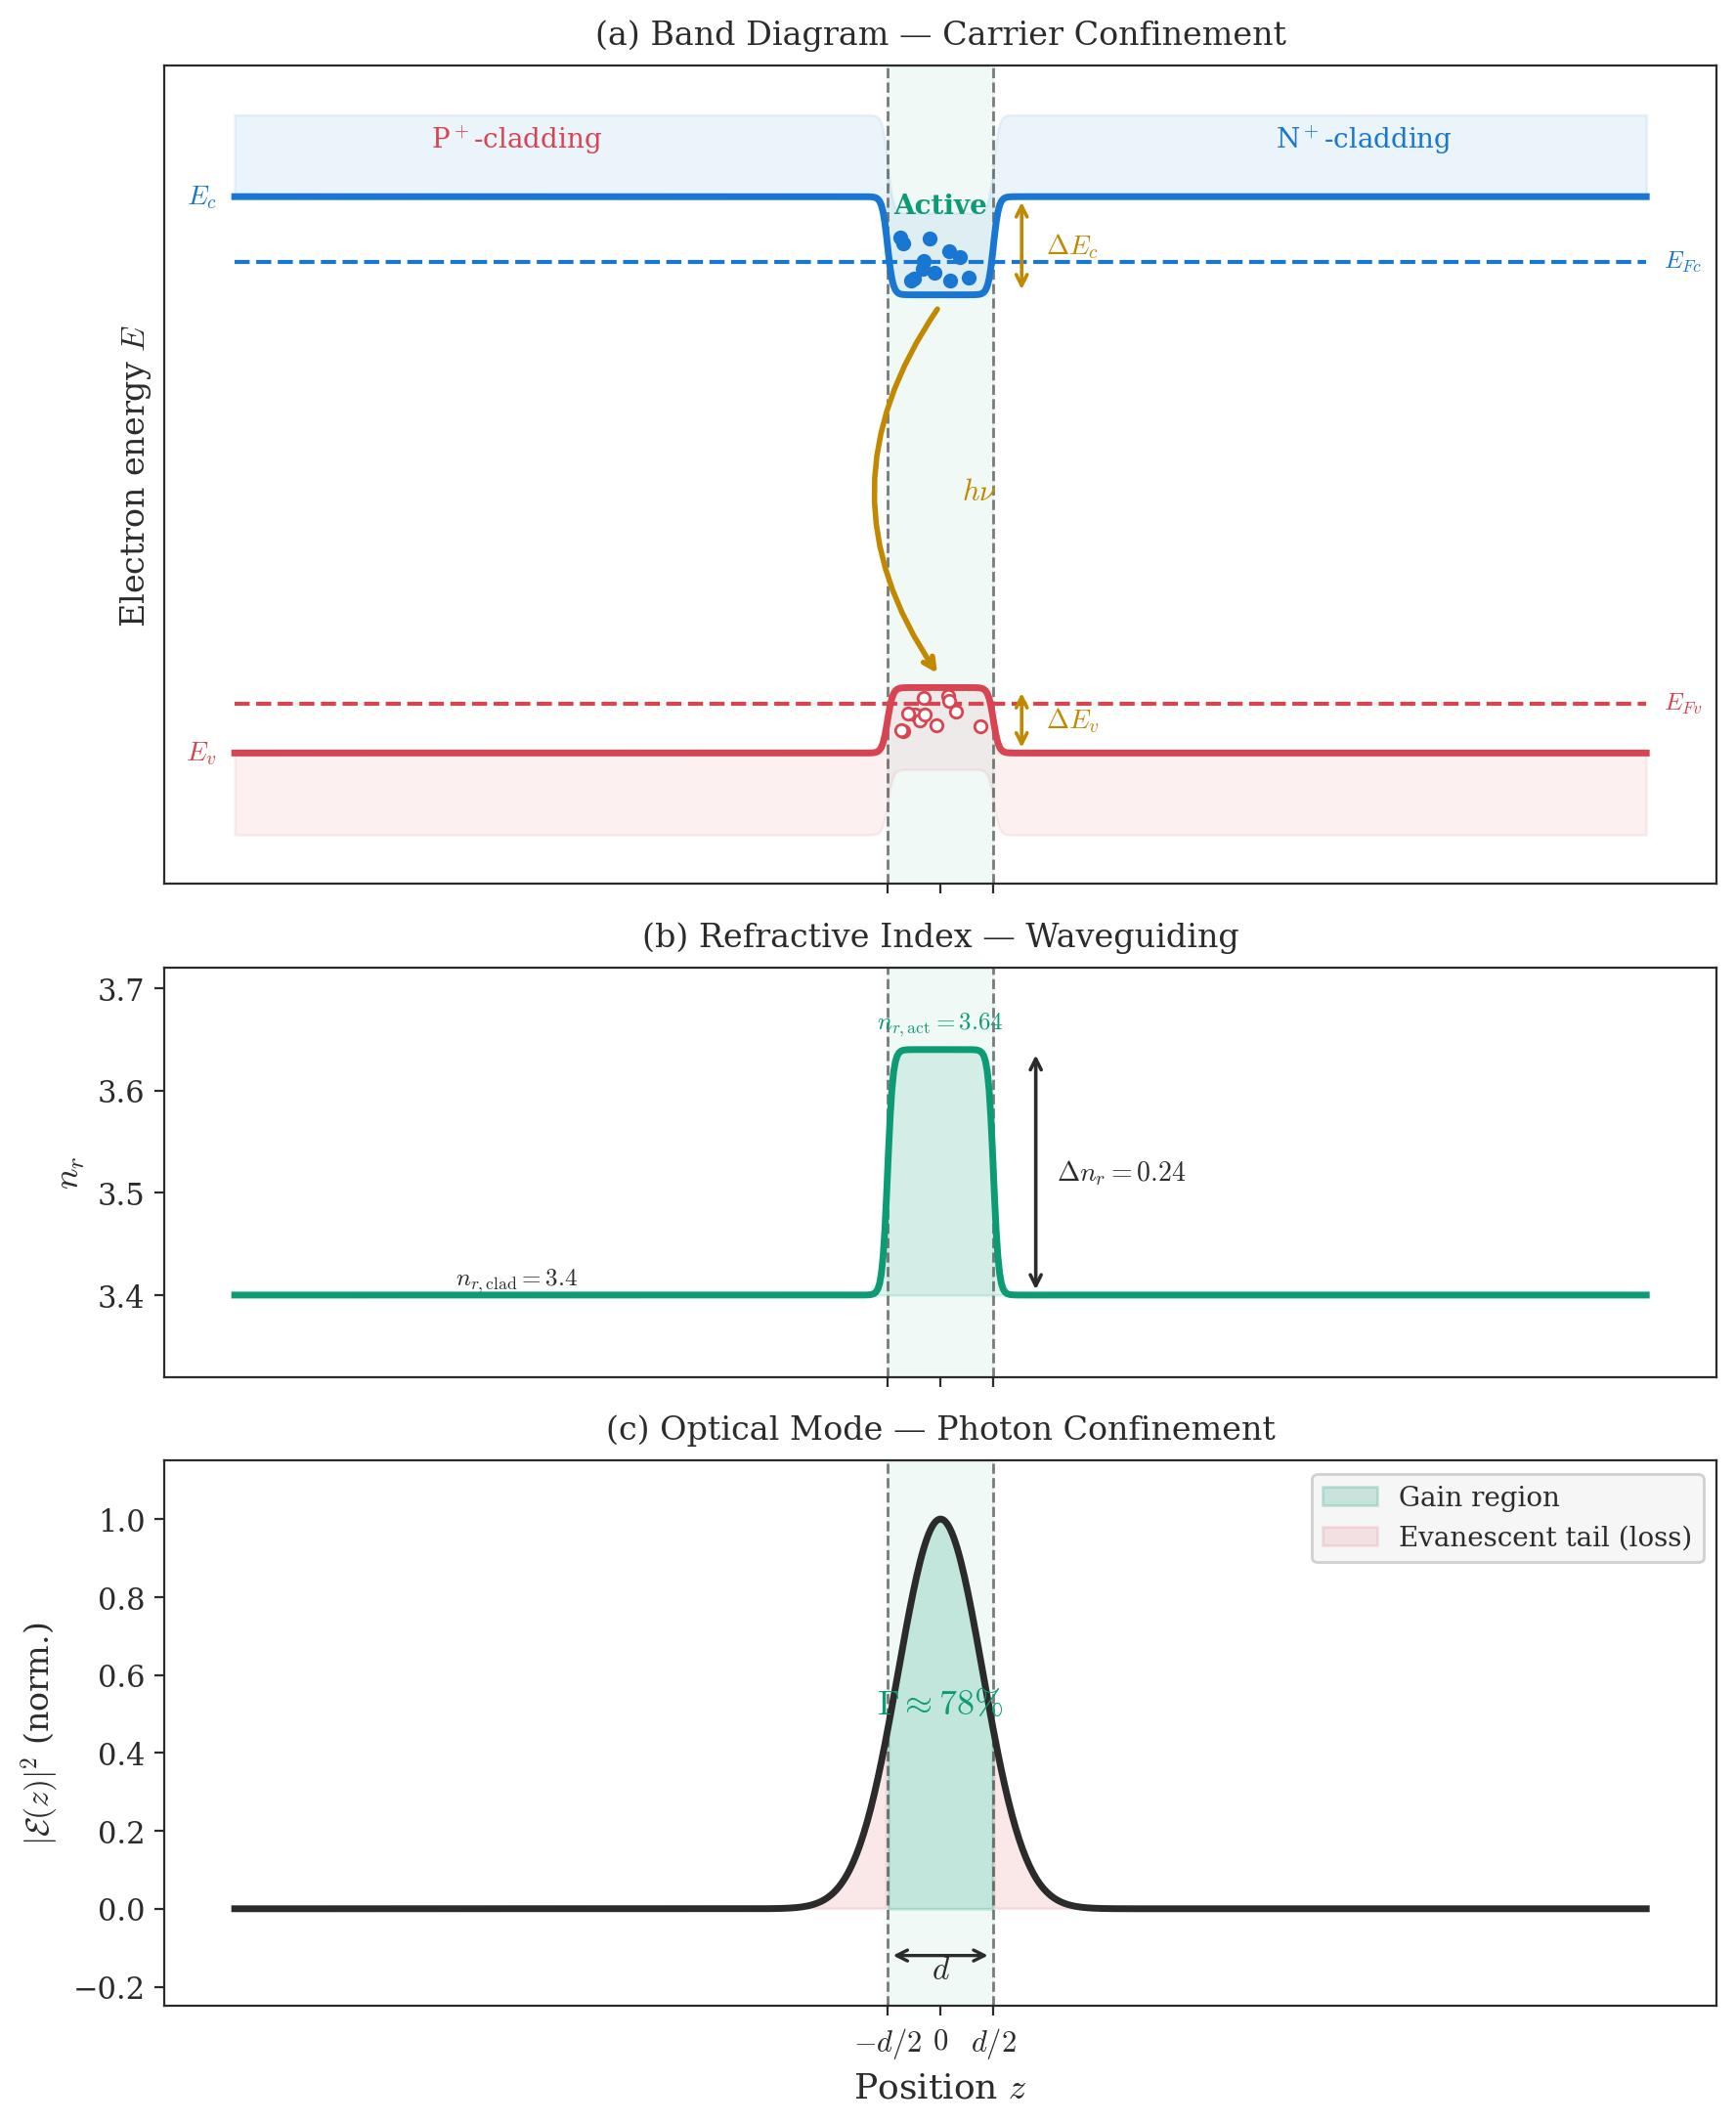
\includegraphics[width=0.75\textwidth]{Figures/Chapter 6/dh_confinement_stacked.jpg}
    \caption{Unified view of the Double Heterostructure: (a) Band diagram showing the quantum well that traps carriers, (b) Refractive index step that creates the waveguide, (c) Resulting optical mode concentrated in the active layer. The same physical boundaries (dashed lines at $\pm d/2$) solve both confinement problems simultaneously.}
\end{figure}

\subsection{Photon Confinement via the Optical Confinement Factor}

The second massive advantage of the double heterostructure is completely optical, and it perfectly complements the carrier confinement. 

By a fortunate twist of semiconductor physics, materials with a smaller bandgap (like our active layer) naturally tend to have a \emph{higher} refractive index than materials with a wider bandgap (like the cladding layers). 

This means that the exact same three-layer sandwich that traps our electrons also forms a perfect \textbf{dielectric waveguide} (essentially a microscopic optical fibre). The high-index active layer acts as the core, and the low-index cladding acts as the reflective boundary. Because of total internal reflection, the generated photons are guided and concentrated almost entirely within the active layer, exactly where the population inversion is happening. 

We quantify this spatial overlap using the \textbf{optical confinement factor} ($\Gamma$), which is the percentage of the optical wave that physically sits inside the gain region. As shown in the previous figure, a well-designed DH laser can achieve $\Gamma \approx 30\% \text{ to } 80\%$, meaning the vast majority of the photon energy is successfully amplified rather than leaking away into the dark, unpumped cladding. 

By confining both the carriers \emph{and} the photons to the exact same microscopic volume, the DH laser operates with extreme efficiency, dropping the required threshold current by a massive factor compared to a homojunction.

\subsection{Materials Design: Lattice Matching}

When growing a semiconductor heterostructure, we face one absolute physical constraint: the distance between atoms in the adjoining materials must be nearly identical. This fundamental atomic spacing is called the \textbf{lattice constant}.

If we attempt to grow a material with a larger lattice constant on top of one with a smaller lattice constant, the top layer must physically squeeze its atomic bonds to align with the substrate. This creates immense mechanical strain. If the mismatched layer is grown thicker than a few nanometres, the accumulated strain becomes unbearable and the crystal structure ``snaps,'' creating missing planes of atoms known as \textbf{misfit dislocations}. In optoelectronics, dislocations are catastrophic. They act as deep trap states in the middle of the bandgap, capturing electrons and holes and forcing them to recombine non-radiatively (producing heat instead of light), which completely destroys the laser's efficiency. 

The visual map below illustrates how we navigate this strict constraint by plotting the bandgap against the lattice constant. 

The most famous success story is the near-infrared system: Al$_x$Ga$_{1-x}$As grown on a GaAs substrate. By substituting Aluminum for Gallium, we can freely increase the bandgap. As shown by the nearly vertical solid black line in the map, this compositional tuning barely changes the lattice constant (the mismatch is less than 0.15\%). This makes AlGaAs the ``holy grail'' of heterostructures: we can arbitrarily tune the bandgap to create our confinement barriers without ever inducing crystal strain. For $x \lesssim 0.45$, the bandgap is direct and varies linearly:
\begin{equation*}
    E_g(\text{Al}_x\text{Ga}_{1-x}\text{As}) \approx 1.424 + 1.247x \quad [\text{eV}]
\end{equation*}

However, for long-haul telecommunications ($1.55\,\mu$m), we require a much smaller bandgap ($\approx 0.75\,\text{eV}$) to hit the minimum-loss window of silica optical fibres. The material of choice is InGaAs. But unlike Aluminum, adding Indium violently expands the lattice constant. As the blue curves in the map demonstrate, we cannot pick our composition freely. We are forced to carefully engineer the alloy to the exact composition of In$_{0.53}$Ga$_{0.47}$As so that its lattice constant perfectly intersects the vertical dashed line of an InP substrate. This exact mixture guarantees a defect-free interface while simultaneously hitting the critical telecom wavelength.

\begin{figure}[H]
    \centering
    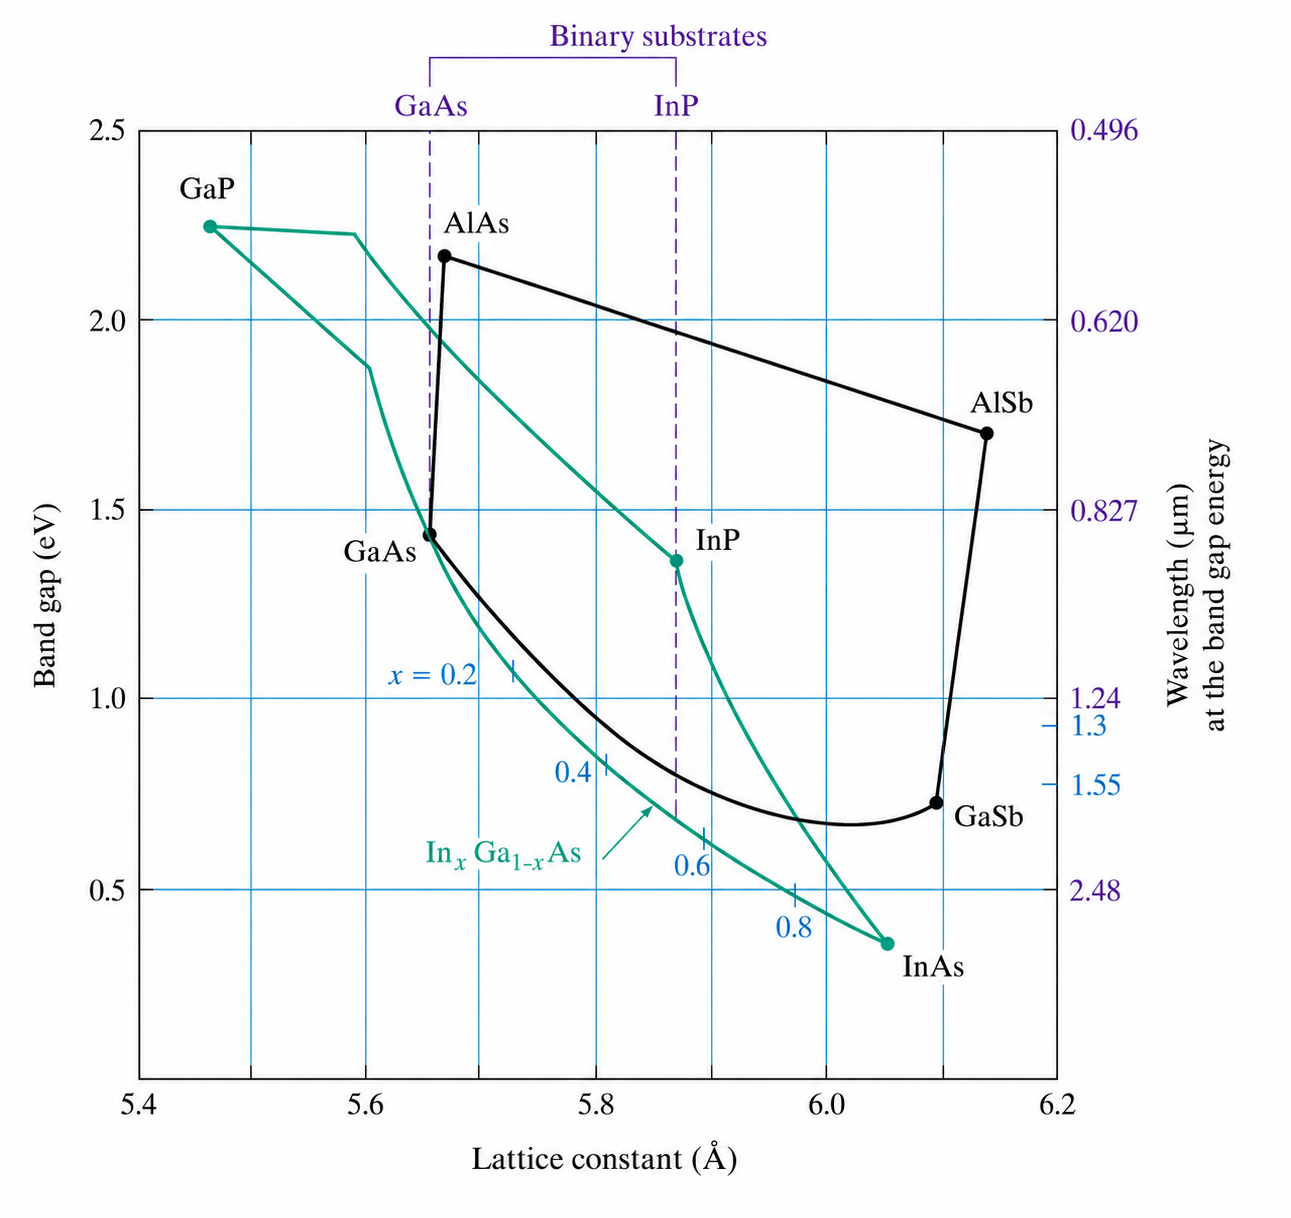
\includegraphics[width=0.65\textwidth]{Figures/Chapter 6/lattice_matching_map.jpg}
    \caption{Bandgap vs. Lattice Constant map for III-V Semiconductors. Vertical alignment indicates perfect lattice-matching (e.g., AlAs on GaAs, or In$_{0.53}$Ga$_{0.47}$As on InP), while the solid curves show how ternary alloys bridge the gaps.}
\end{figure}

\begin{keyinsight}[The DH Laser as a Stepping Stone]
    The double heterostructure solved the two critical problems of the homojunction — thick gain regions and weak optical confinement — through a single architectural innovation. The AlGaAs/GaAs material system made this practically realisable with nearly perfect lattice matching. These same two confinement principles — carrier confinement via band-edge discontinuities and photon confinement via the refractive index step — carry forward unchanged into the quantum well laser. The only thing that changes is the scale: as $d$ shrinks below $\sim 10\,\text{nm}$, the physics transitions from classical 3D semiconductor mechanics to genuine quantum mechanics. The resulting quantum well laser achieves dramatically lower threshold currents and higher differential gain than any bulk DH device, and forms the basis of virtually every practical semiconductor laser built today.
\end{keyinsight}

The next step in this series is to examine what happens to the gain spectrum, threshold current, and efficiency when we shrink the active layer into the quantum confinement regime — and why the quantum well laser has become the dominant architecture in every area from consumer electronics to fibre-optic communications.
